\chapter{一维Tent映射的状态网络分析}

\section{定点域上Tent映射的性质分析}

\subsection{数字化Tent映射的定义}

Tent映射在数学中是指一种分段的线性映射,因其函数图像看似帐篷而得名,其数学表达式为
\begin{equation}
f(x)=\mu \cdot\left(1-2\left|x-1/2\right|\right),
\label{eq:Tent}
\end{equation}
其中$x\in [0,1]$,$\mu\in (0,1]$。Tent映射和Logistic映射实质上是拓扑共轭。

在精度为$n$的定点运算域上,Tent映射
$f(x)=\mu \cdot\left(1-2\left|x-1/2\right|\right)$变为
\begin{equation}
f_n(i)=\left( (N_{\mu}/2^{n_\mu}) \cdot (1-2\left|(i/2^n)-1/2\right|) \right).
\label{eq:TentFinite}
\end{equation}

图~\ref{fig:networkTent5and6bits}为相同控制参数,不同运算精度下Tent映射的状态映射网络$F^\star_n$。

\begin{figure}[!htb]
\centering
\begin{minipage}{0.87\BigTwoImW}
\centering
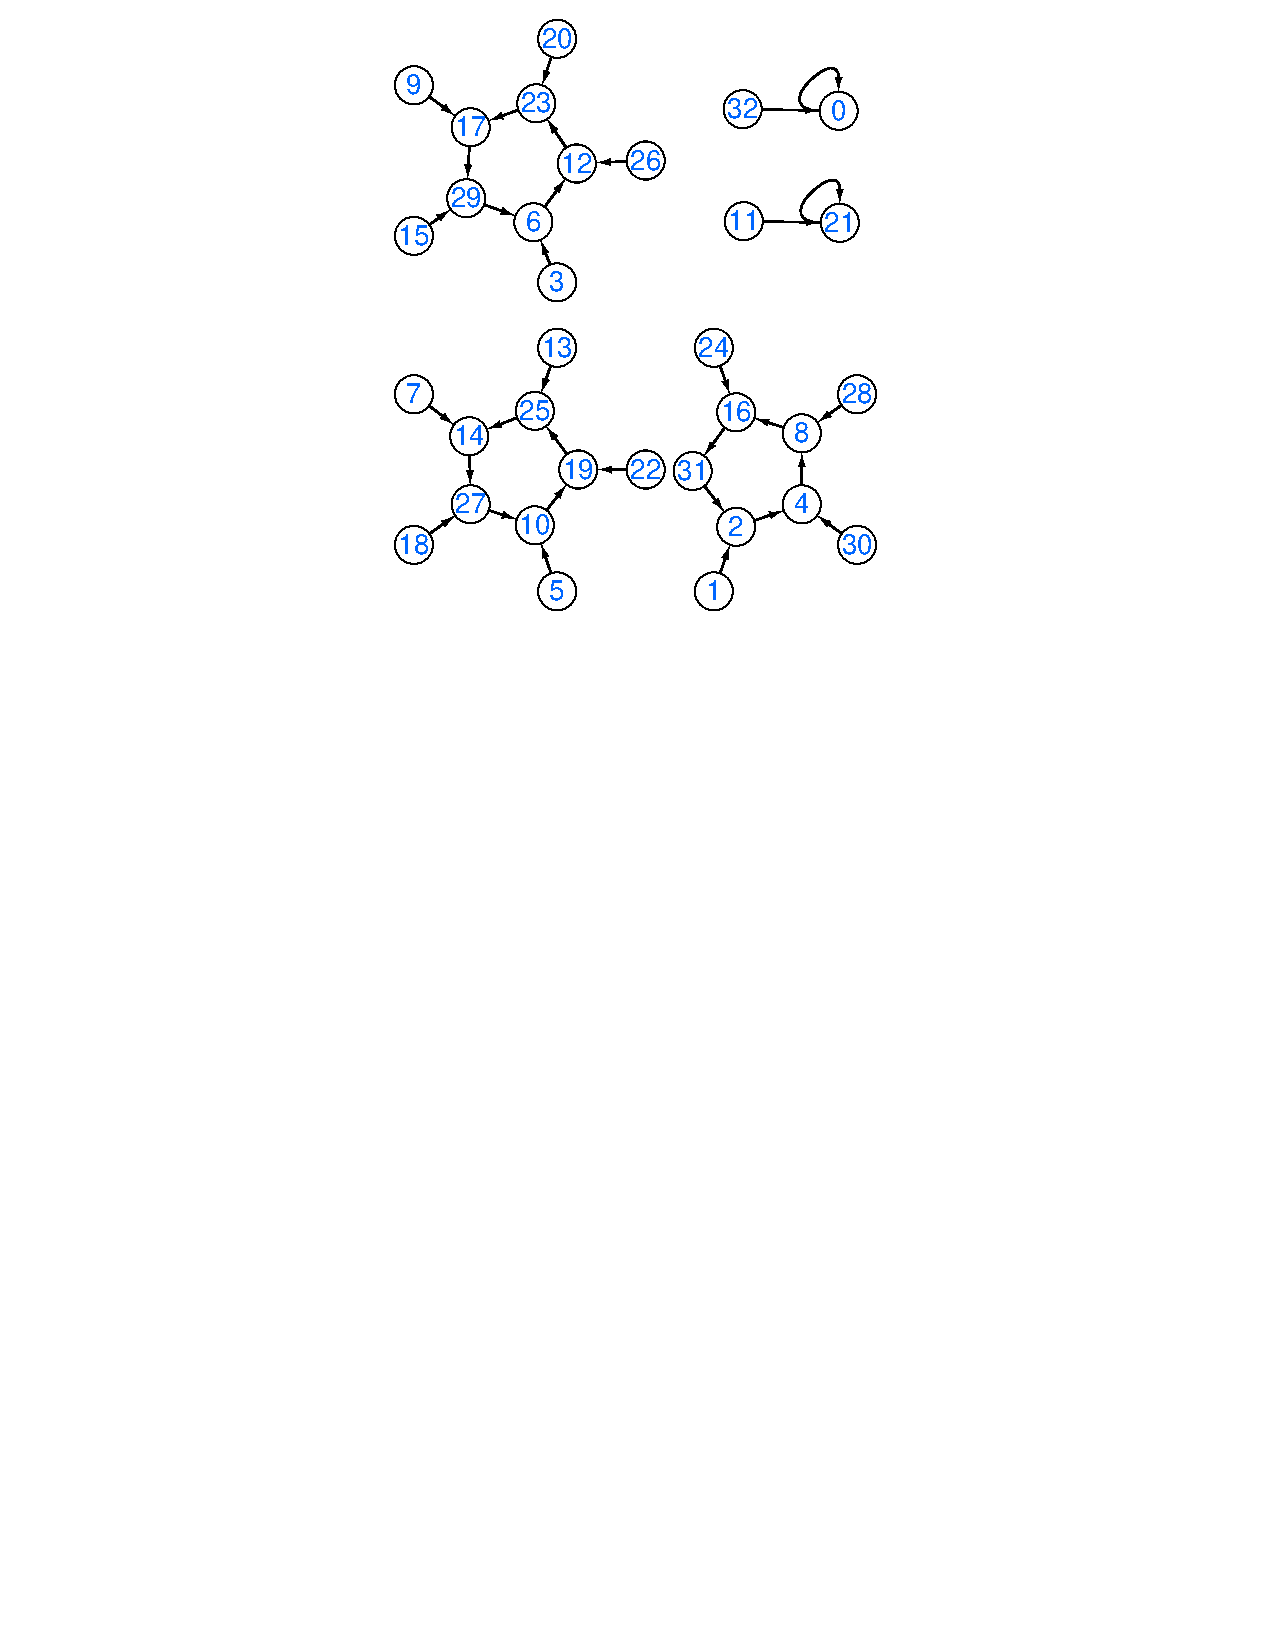
\includegraphics[width=0.87\BigTwoImW]{5_bit_precision_tent}
a)
\end{minipage}\hspace{\figsep}
\begin{minipage}{\BigTwoImW}
\centering
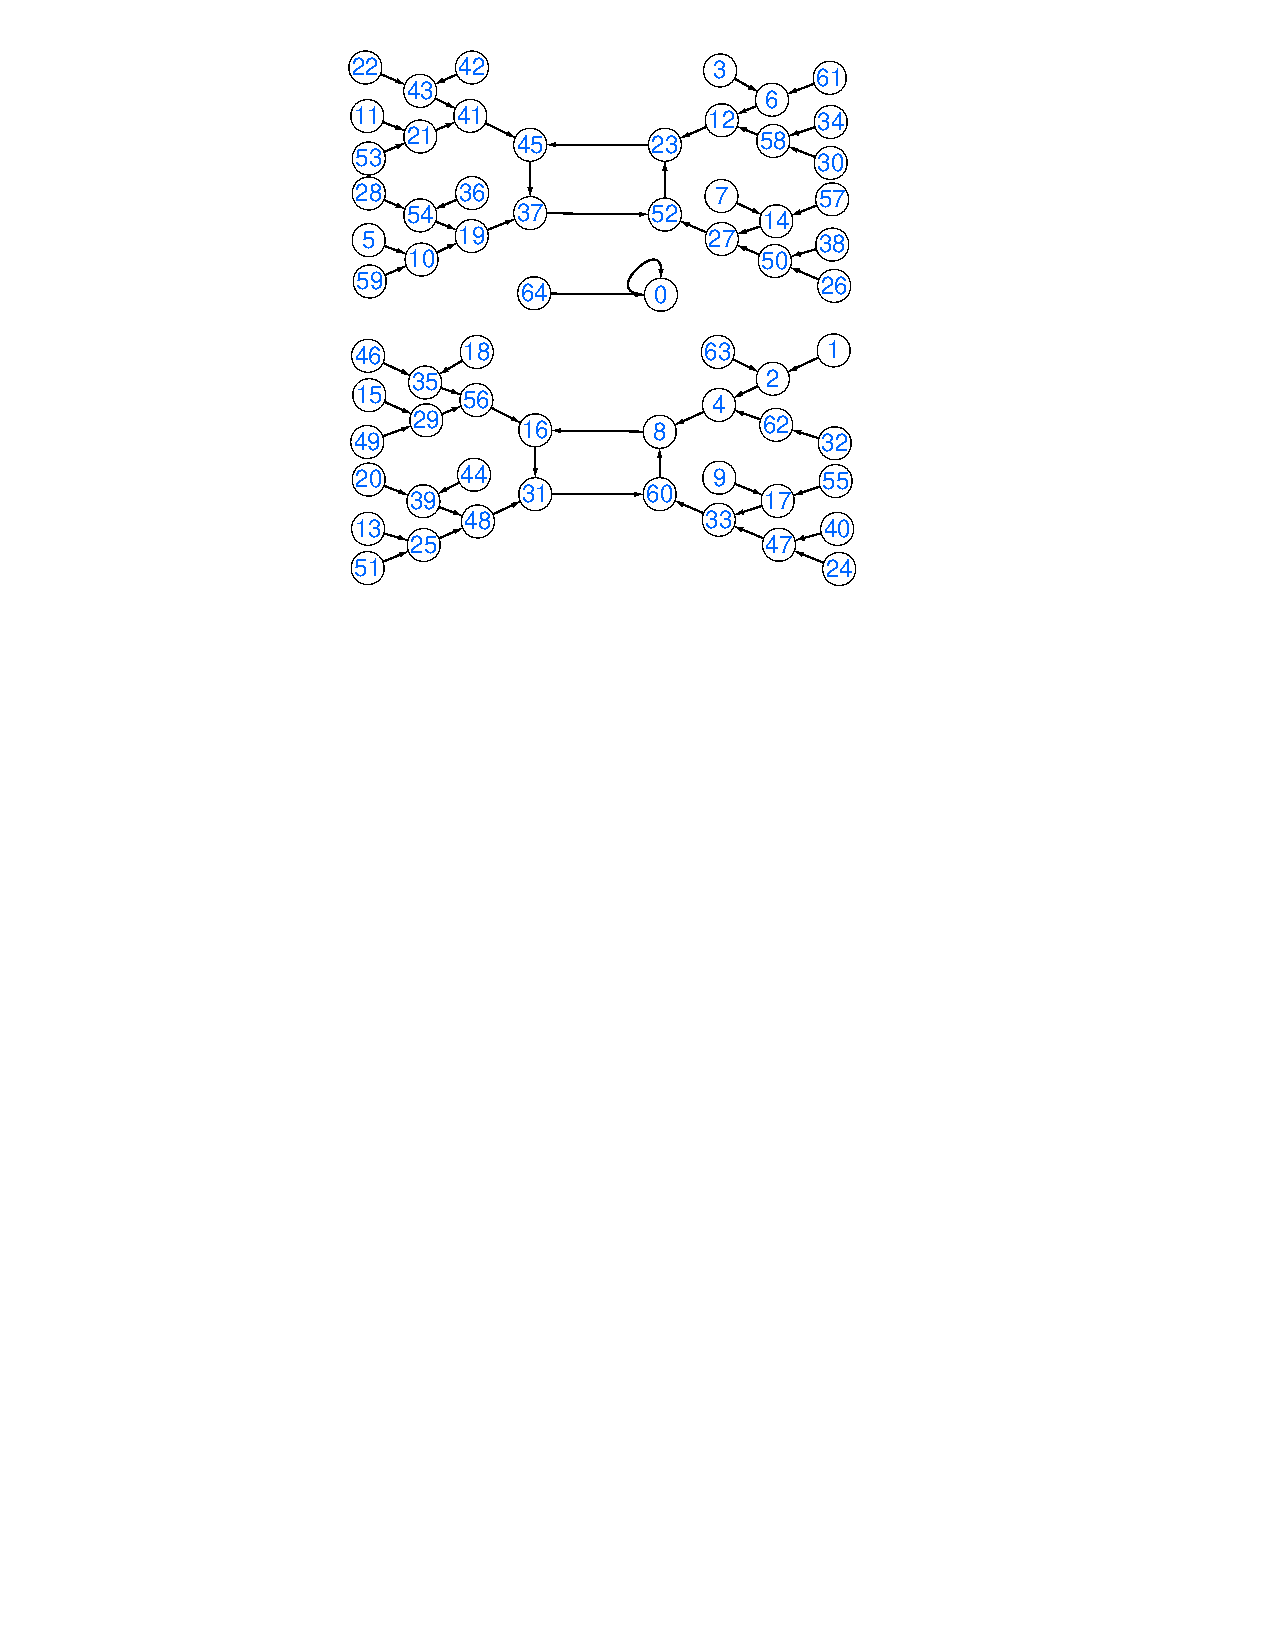
\includegraphics[width=\BigTwoImW]{6_bit_precision_tent}
b)
\end{minipage}
\caption{控制参数$\mu=31/2^5$时,Tent映射的状态映射网络:
a) 5比特精度; b) 6比特精度}
\label{fig:networkTent5and6bits}
\end{figure}

\begin{figure}[!htb]
\centering
\begin{minipage}{0.93\BigTwoImW}
\centering
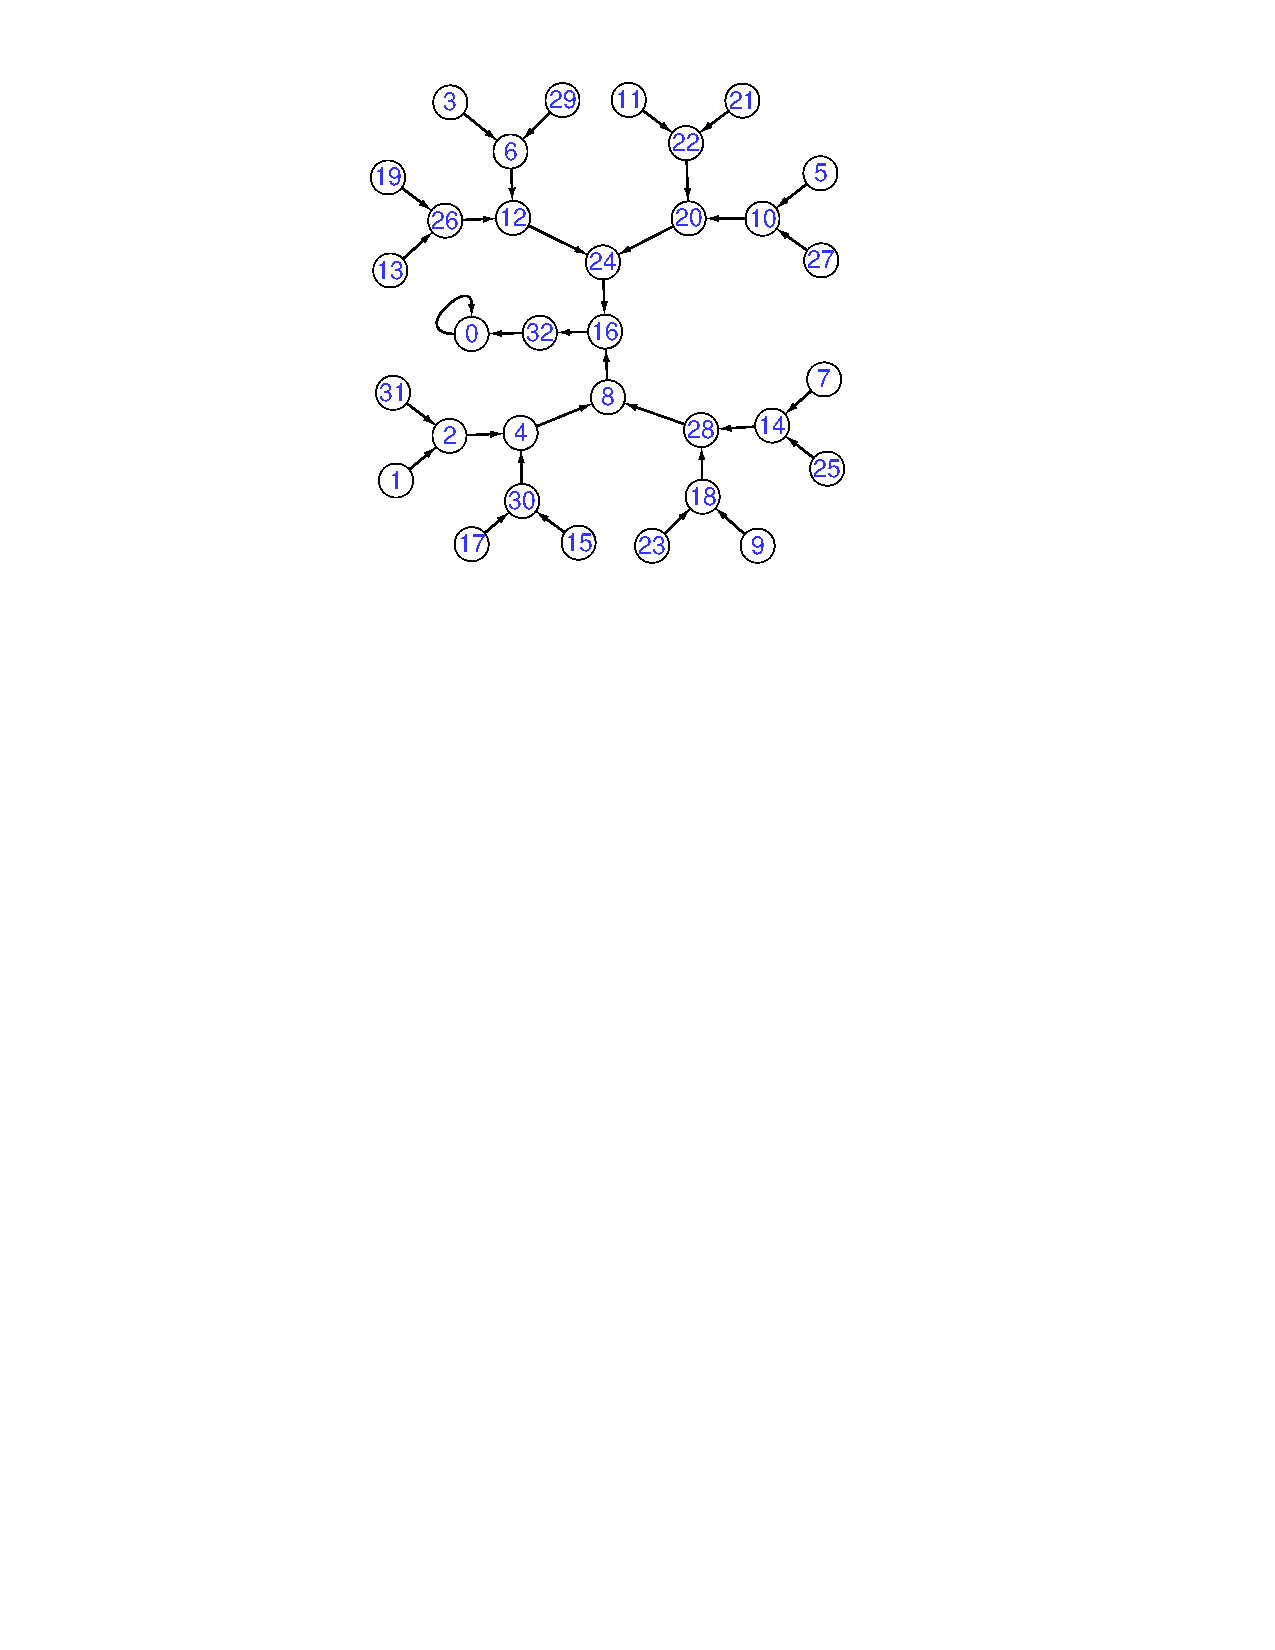
\includegraphics[width=0.93\BigTwoImW]{5_bit_precision_tent_u1}
a)
\end{minipage}\hspace{\figsep}
\begin{minipage}{\BigTwoImW}
\centering
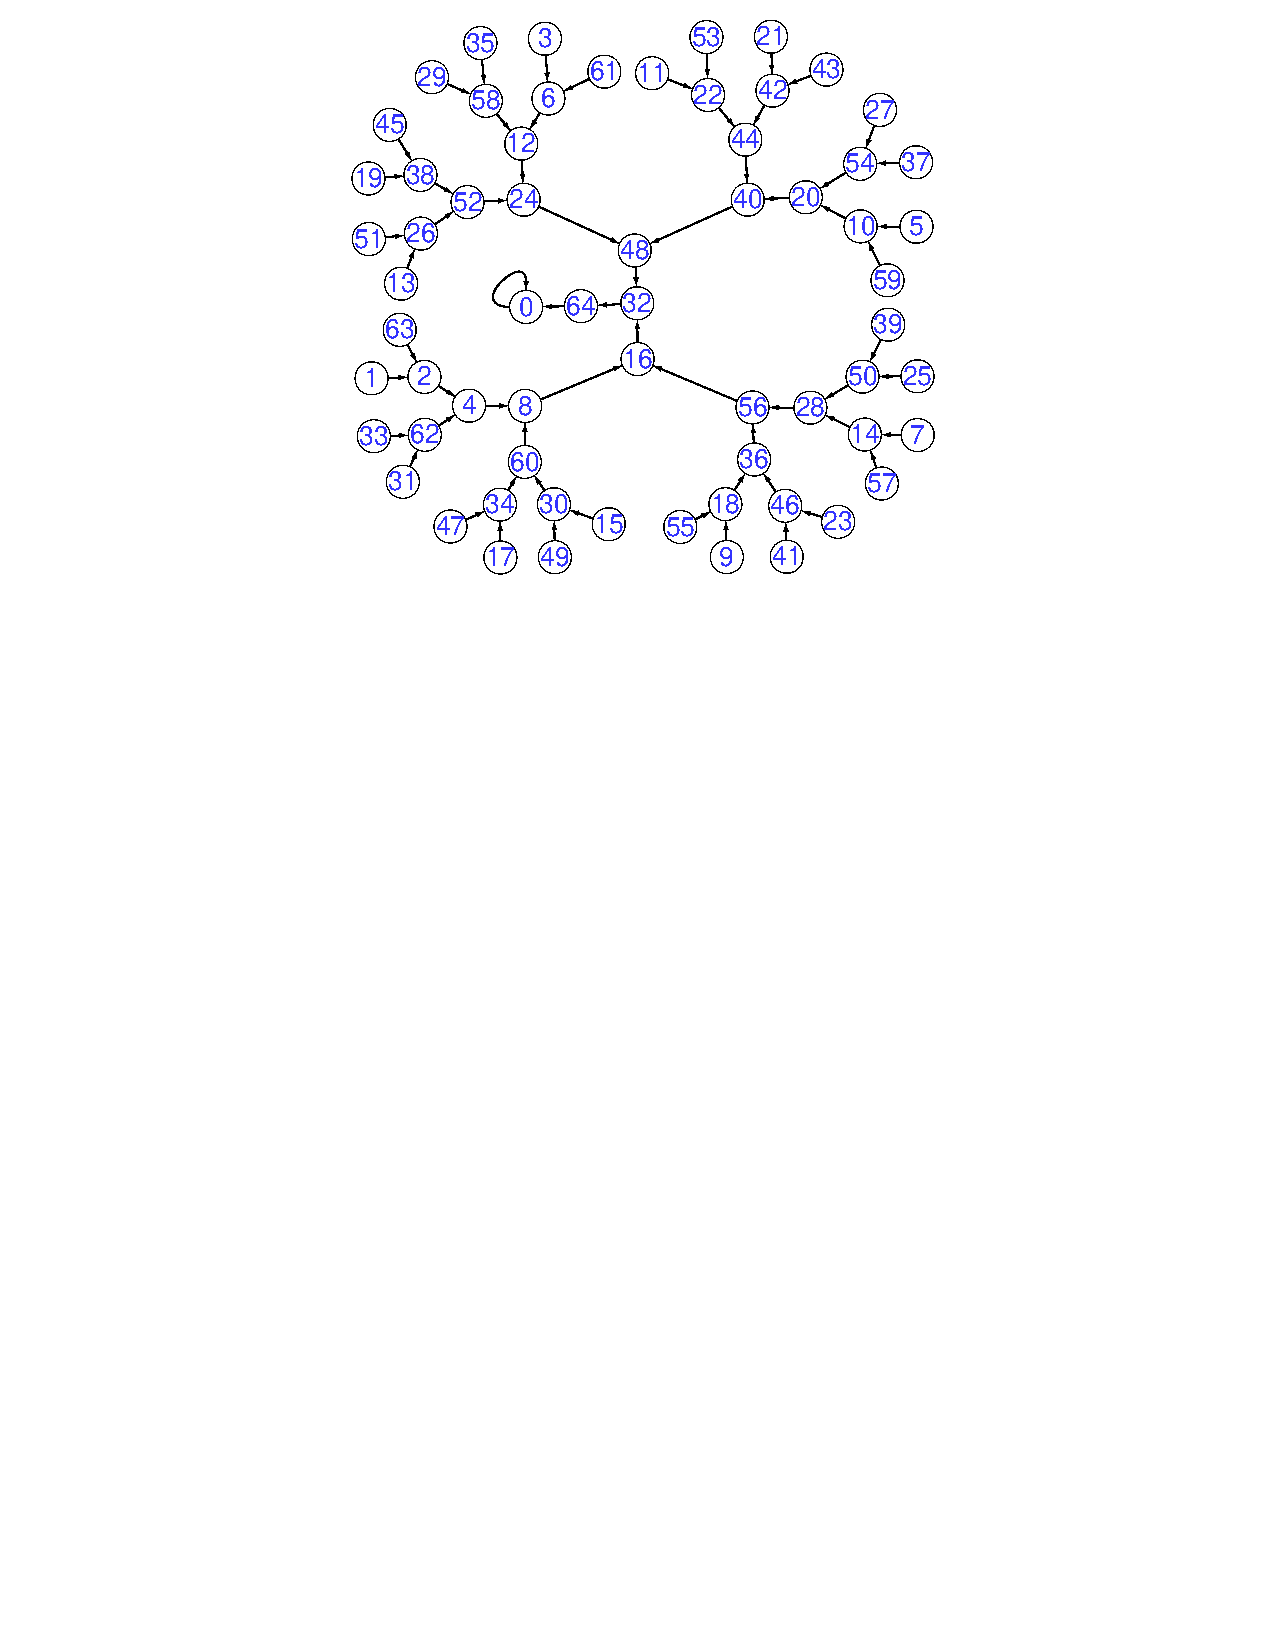
\includegraphics[width=\BigTwoImW]{6_bit_precision_tent_u1}
b)
\end{minipage}
\caption{控制参数$\mu=1$时,Tent映射的状态映射网络:
a) 5比特精度; b) 6比特精度}
\label{fig:networktent5and6bitsu1}
\end{figure}

\subsection{Tent映射的状态映射网络与实现精度之间的关系}

\begin{Corollary}
\label{coro:tentoddUpper}
$F^\star_{n+1}$中节点$(2i+1)$和$F^\star_{n}$中节点$i$满足关系
\begin{equation*}
\left|F^\star_{n+1}(2i+1)-2\cdot F^\star_n(i)\right|\le
\begin{cases}
4  & r_n \in [0.25, 0.75);\nonumber\\
3  & \mbox{其他},
\end{cases}
\end{equation*}
其中$i\in \{0, \cdots, 2^n-1\}$。
\end{Corollary}

\begin{proof}
因为$\left(N_{\mu}/2^{n_\mu-1}\right)\in[0,2]$,将等式~(\ref{eq:TentFinite})代入
不等式~(\ref{eq:oddCondition}),可得
\begin{eqnarray}
\left|F^\star_{n+1}(2i+1)-2\cdot F^\star_n(i)\right|
& \le & \left|\mathrm{R}\left(N_{\mu}/2^{n_\mu-1}\right)\right|+
\begin{cases}
2  & r_n \in [0.25, 0.75);\nonumber\\
1  & \mbox{其他},
\end{cases}\\
& \le  &
\begin{cases}
4  & r_n \in [0.25, 0.75);\nonumber\\
3  & \mbox{其他}.
\end{cases}
\end{eqnarray}\qedsymbol
\end{proof}

\begin{figure}[!htb]
\centering
\begin{minipage}{\TwoImW}
\centering
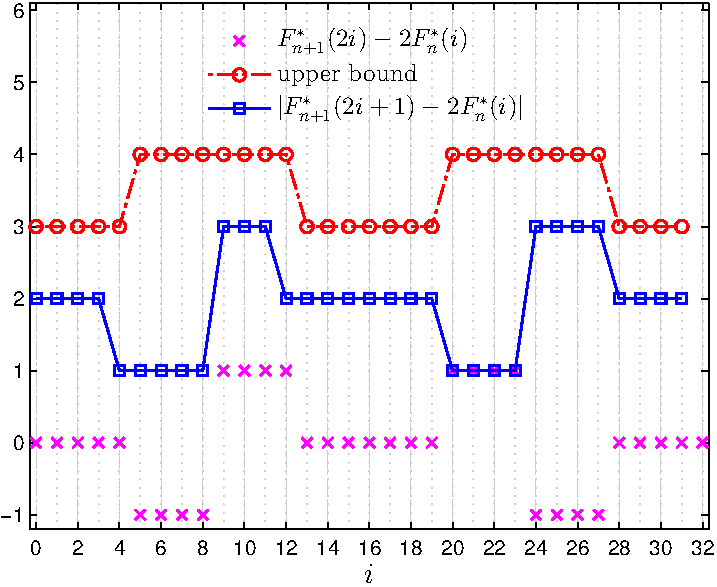
\includegraphics[width=\TwoImW]{upper_bound_add_tent}
a)
\end{minipage}
\begin{minipage}{\TwoImW}
\centering
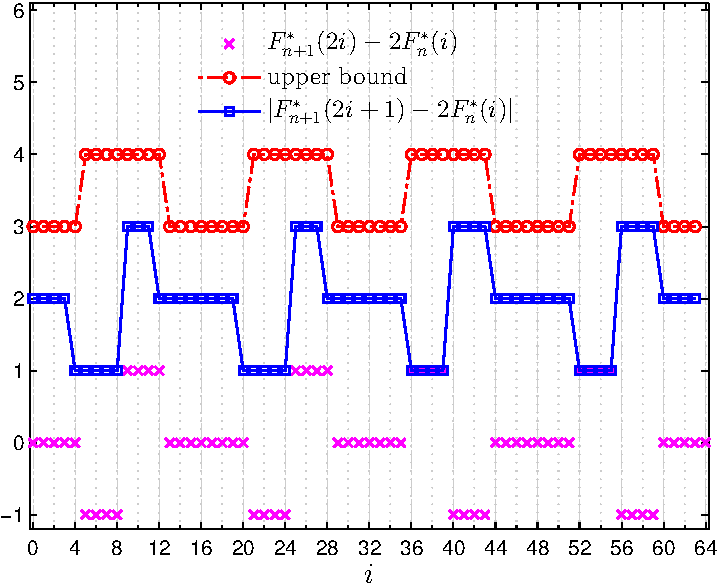
\includegraphics[width=\TwoImW]{upper_bound_add_tent2}
b)
\end{minipage}
\caption{$F^\star_{n}$与$F^\star_{n+1}$中对应节点的差值分布: a) $n=5$; b) $n=6$}
\label{fig:upperboundtent}
\end{figure}

根据推论~\ref{coro:tentoddUpper}可知,$|F^\star_{n+1}(2i+1)-2\cdot F^\star_n(i)|$的上界仅仅取决于$N_{\mu}$。
图~\ref{fig:upperboundtent} a)为图~\ref{fig:networkTent5and6bits} a)中每个节点对应的差值
$|F^\star_{n+1}(2i+1)-2\cdot F^\star_n(i)|$和$F^\star_{n+1}(2i)-2F^\star_n(i)$,类似地,
为进一步分析比较$F^*_{n}$和$F^*_{n+1}$的关系,图~\ref{fig:networkTent5and6bits} b)中每个节点
对应的差值如图~\ref{fig:upperboundtent} b)所示。

\subsection{Tent映射SMN入度分布的理论推导}

\begin{Property}
\label{prop:degree}
Tent映射对应状态映射网络的节点入度仅有三种可能取值:
\begin{equation*}
k=
\begin{cases}
1  & \mbox{\rm 最大值对应节点;}\\
2  & \mbox{\rm 其他具有原像的节点;}\\
0  & \mbox{\rm 其他节点.}
\end{cases}
\end{equation*}
\end{Property}
\iffalse
\begin{Property}
\label{prop:degree}
Tent映射对应状态映射网络的节点入度仅有三种可能取值:1,2,3。
\end{Property}\fi
\begin{proof}
当$x=1/2$时,$f(x)=\mu$取最大值。$x=1/2$所在区间对应节点唯一指向$y=\mu$所在区间对应节点,
因此$y=\mu$所在区间对应节点的入度$k=1$。

由于Tent映射具有对称性,这里只考虑定义域的左半部分。Tent映射$y=f(x)$的反函数为
\begin{equation*}
f^{-1}(y)=y/\left( 2\mu \right),\ x\in [0, 1/2].
\end{equation*}

当$x\in [0,1/2]$时,$f'(x)=2\mu>0$,$f(x)$关于$x$单调递增。根据定理~\ref{theorem:logisticMap}的
证明可知,$y\neq \mu$所在区间对应节点的入度为
\begin{eqnarray*}
k &=& 2\cdot \left\lceil \frac{f^{-1}(y)-f^{-1}(y-(1/2^{n}))}{2^{-n}} \right\rceil\\
  &=& 2\cdot \left\lceil \frac{y/(2\mu)-(y-1/2^{n})/(2\mu)}{2^{-n}} \right\rceil  \\
  &=& 2\cdot \left\lceil 1/(2\mu) \right\rceil\\
  &=& 2.
\end{eqnarray*}

由此上述关于Tent映射的状态映射网络入度分布的性质得以证明,即Tent映射对应状态映射网络的节点入度仅有三种可能取值:1,2,3。\qedsymbol
\end{proof}

\begin{figure}[!htb]
\centering
\begin{minipage}{\TwoImW}
\centering
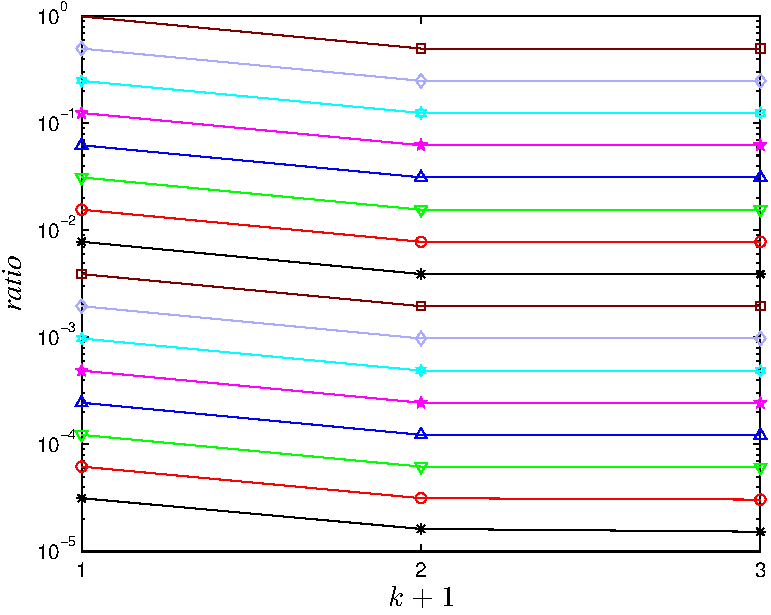
\includegraphics[width=\TwoImW]{CumulativeInDegreeDistribution_u31_n_5_20}
a)
\end{minipage}
\begin{minipage}{\TwoImW}
\centering
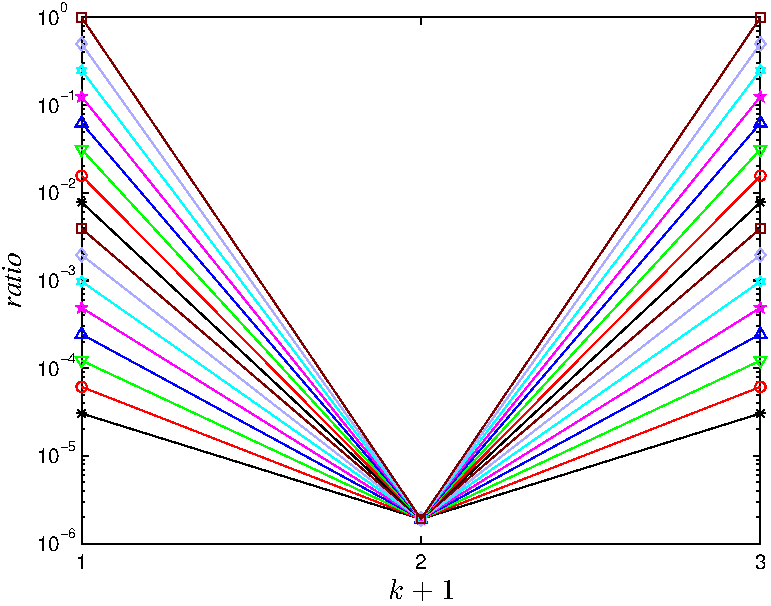
\includegraphics[width=\TwoImW]{InDegreeDistribution_u31_n_5_20}
b)
\end{minipage}
\caption{控制参数$\mu=31/2^5$时,状态映射网络$F^\star_{5} \sim F^\star_{20}$的节点度分布:
a) 累积入度分布; b) 入度分布}
\label{fig:InDegreeDistribution3}
\end{figure}

根据性质~\ref{prop:degree}可知,Tent映射对应状态映射网络的节点入度不会随着运算精度的增加而累积
(详见图~\ref{fig:InDegreeDistribution3}),这与Logistic映射不同。

基于上述讨论,可以得出结论:$f''(x)>0$是混沌映射对应状态映射网络的节点入度满足幂律分布的充分而非必要条件。

\section{浮点域上Tent映射的性质分析}

假设Tent映射的迭代初值$x(0)=(0.b_1b_2\cdots b_j\cdots b_{L-1}b_L)_2\neq 0$,其中$b_L=1$(最低有效位),
则$1-x(0)=(0.b_1'b_2'b_3'\cdots b_j'\cdots b_{L-1}'b_L)_2$。根据上述假设,可得
\begin{equation*}
x(1)=\begin{cases} 2x(0)=x(0)\ll 1=(0.b_2\cdots b_j\cdots b_{L-1}b_L)_2  &  0\leq x(0)<0.5;\\
2(1-x(0))=(b_1'.b_2'b_3'\cdots b_j'\cdots b_{L-1}'b_L)_2                 &  0.5\leq x(0)\leq 1,
\end{cases}
\end{equation*}
其中$\ll$表示左移运算。
注意到,当$0\leq x(0)<0.5$时,$b_1=0$。Tent映射迭代$L-1$次,有$x(L-1)\equiv(0.b_L)_2=(0.1)_2$,
进而可知$x(L)\equiv 1$,$x(L+1)\equiv 0$,即$x$趋于0所需迭代次数为$N_r=L+1$。特别地,当$x(0)=0$时,$N_r=0$。
以图~\ref{fig:networkTent7and8bitsu1} a)中节点$``13"$为例,Tent映射的迭代过程如下:
$(0.01101)_{2}\rightarrow (0.1101)_{2}\rightarrow (0.011)_{2}\rightarrow
(0.11)_{2}\rightarrow (0.1)_{2}\rightarrow (1)_{2}\rightarrow (0)_{2}$。

\begin{figure}[!htb]
\centering
\begin{minipage}{\BigTwoImW}
\centering
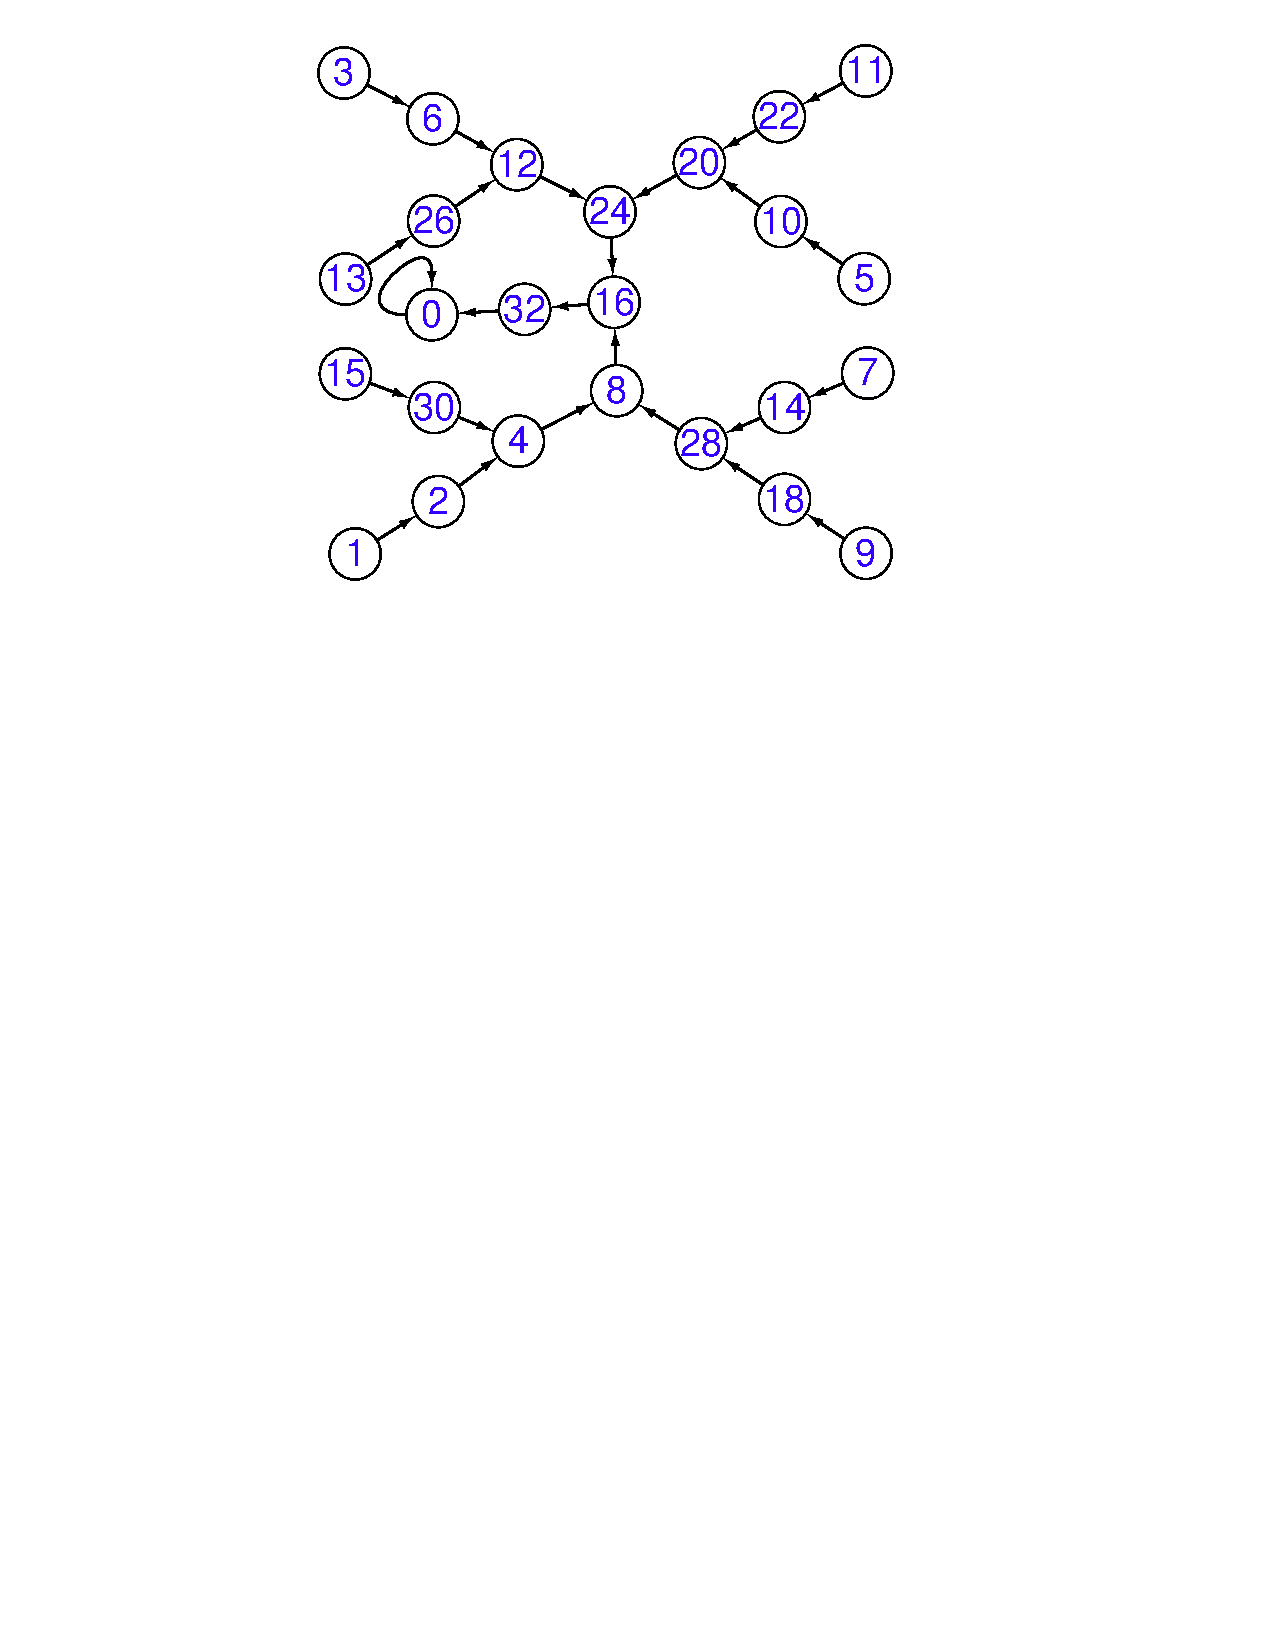
\includegraphics[width=\BigTwoImW]{7bit_out_index_data_tent_u1}
a)
\end{minipage}
\begin{minipage}{\BigTwoImW}
\centering
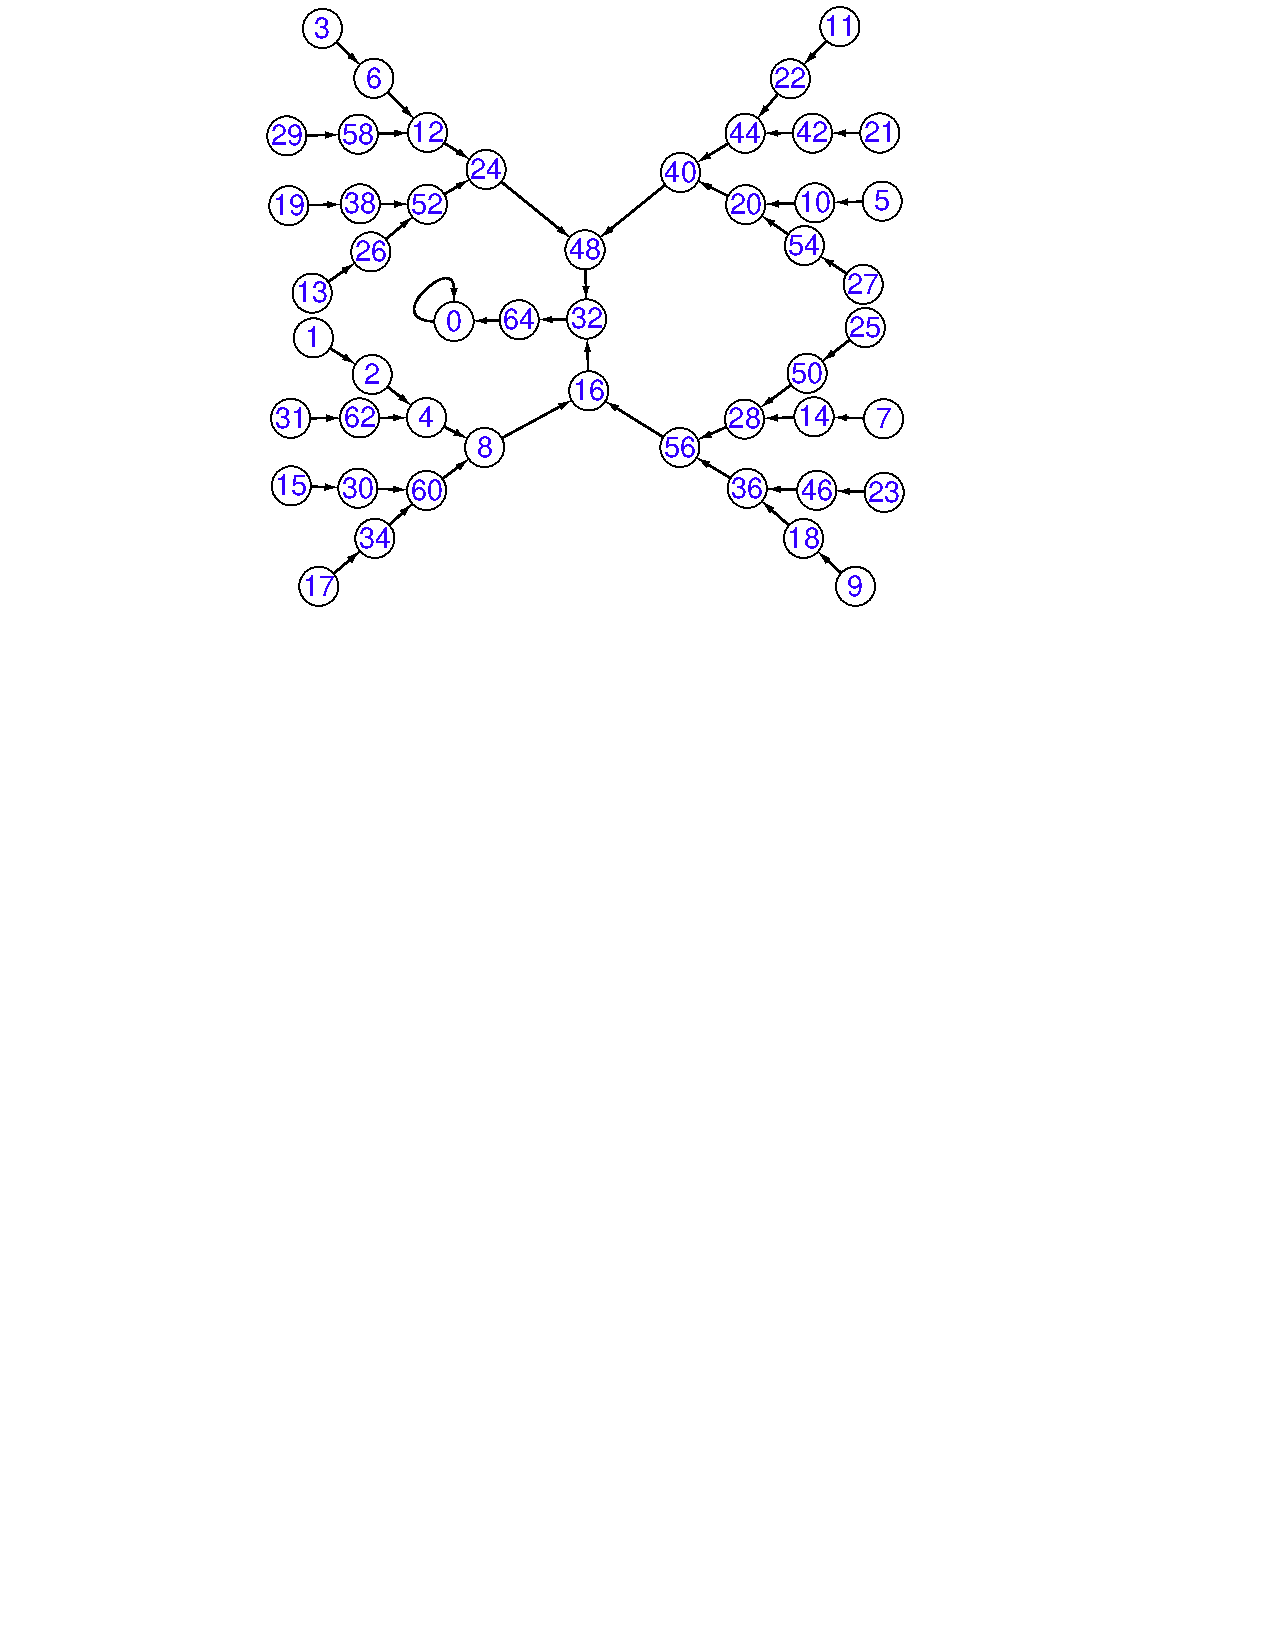
\includegraphics[width=\BigTwoImW]{8bit_out_index_data_tent_u1}
b)
\end{minipage}
\caption{控制参数$\mu=1$时,浮点运算域上Tent映射的状态映射网络:
a) $(l,m)=(3,3)$; b) $(l,m)=(3,4)$}
\label{fig:networkTent7and8bitsu1}
\end{figure}

通常在数字混沌系统的迭代过程中不可避免地要引入量化误差,这种系统量化误差会使数字混沌系统的混沌轨道变得异常复杂且难以预测,进而偏离连续域上混沌系统的实际混沌轨道。
根据上述分析过程可知,$\mu=1$时,Tent映射~(\ref{eq:Tent})的迭代过程可利用左移运算$\ll$在计算机上准确执行,不会引入任何量化误差。
有效数位$L$的值可根据$x(0)\neq 0$的表示形式来确定:
\begin{itemize}

\item 当$x(0)$为规格化数:
$x(0)=(1.b_{m-1}\cdots b_{0})\times 2^{-e}
=(0.\overbrace{0\cdots 0}^{e-1}1b_{m-1}\cdots b_{0})_{2}$。
假设$x(0)$的最低有效位为$b_{i}=1$,则$x(0)=(0.\overbrace{0\cdots 0}^{e-1}1\overbrace{b_{m-1}\cdots
b_{i}}^{m-i}\overbrace{0\cdots 0}^{i})_{2}$,$L=(e-1)+1+(m-i)=e+(m-i)$。
当$e\in [1,2^{l-1}-2]$,$i\in [0,m-1]$时,$L\in [2, 2^{l-1}-2+m]$;

\item 当$x(0)$为非规格化数:
$x(0)=(0.b_{m-1}\cdots b_{0})\times 2^{2-2^{l-1}}
=(0.\overbrace{0\cdots 0}^{2^{l-1}-2}b_{m-1}\cdots b_{0})_{2}$。
假设$x(0)$的最低有效位为$b_{i}=1$,则$x(0)=(0.\overbrace{0\cdots 0}^{2^{l-1}-2}\overbrace{b_{m-1}\cdots
b_{i}}^{m-i}\overbrace{0\cdots 0}^{i})_{2}$,$L=2^{l-1}-2+(m-i)=2^{l-1}-2+m-i$。
当$i\in [0,m-1]$时,$L\in [2^{l-1}-1,2^{l-1}-2+m]$。
\end{itemize}
根据上述讨论可知,无论哪种$x(0)$的表示形式,总有$L \le 2^{l-1}-2+m$。

首先,考虑$i\in \{0,\cdots ,m-1\}$的数学期望。不失一般性,假设
尾数$(b_{m-1}\cdots b_{0})_{2}$在集合$\{0,\cdots ,2^{m}-1\}$上均匀分布\upcite{Math2000Probability},则有
\begin{align*}
\mathit{Prob}[(b_{i}=1,b_{i-1}=\cdots =b_{0}=0)] = & \frac{2^{m-1-i}}{2^{m}} = \frac{1}{2^{i+1}},\\
\mathit{Prob}[(b_{m-1}=\cdots =b_{0}=0)] = & \frac{1}{2^{m}},
\end{align*}
从而可知$i$的数学期望为
\begin{eqnarray*}
E(i) \approx \sum_{i=0}^{m-1} i\cdot \frac{1}{2^{i+1}} + m\cdot \frac{1}{2^{m}}
= \frac{1}{2}\cdot \sum_{i=1}^{m-1} \frac{i}{2^{i}} + \frac{m}{2^{m}}
= 1 - \frac{1}{2^{m}}.
\end{eqnarray*}

下面分析$e\in \{1,\cdots ,2^{l-1}-2\}$的数学期望。根据$x(0)$在区间[0,1]上的均匀分布\upcite{Math2000Probability},可知
\begin{equation*}
\mathit{Prob}[2^{-e}\le x(0) < 2^{-(e-1)}]=2^{-e}.
\end{equation*}
因此$e$的数学期望为
\begin{equation*}
E(e)\approx \sum_{e=1}^{2^{l-1}-2} \frac{e}{2^{e}}=2-\frac{2^{l-1}}{2^{2^{l-1}-2}}\approx 2.
\end{equation*}
根据上述推导,进一步可得
\begin{eqnarray}
E(L)
& =       & \mathit{Prob}[\mathrm{normalized\ numbers}]\cdot \left(E(e)+(m-E(i))\right)+\nonumber\\
&         & \mathit{Prob}[\mathrm{denormalized\ numbers}]\cdot \left(2^{l-1}-2+m-E(i)\right)\nonumber\\
& =       & \frac{2^{l-1}-2}{2^{l-1}-1}\cdot \left(E(e)+(m-E(i))\right)+\nonumber\\
&         & \frac{1}{2^{l-1}-1}\cdot \left(2^{l-1}-2+m-E(i)\right)\nonumber\\
& \!\approx\! & \frac{2^{l-1}-2}{2^{l-1}-1}\cdot (2+(m-1))\!+\! \frac{1}{2^{l-1}-1}\cdot (2^{l-1}-2+m-1)\nonumber\\
& =       & \frac{(2^{l-1}-2)(m+2)+m-1}{2^{l-1}-1}.
\label{eq:EL}
\end{eqnarray}

\begin{figure}[!htb]
\centering
\begin{minipage}{1.25\BigOneImW}
\centering
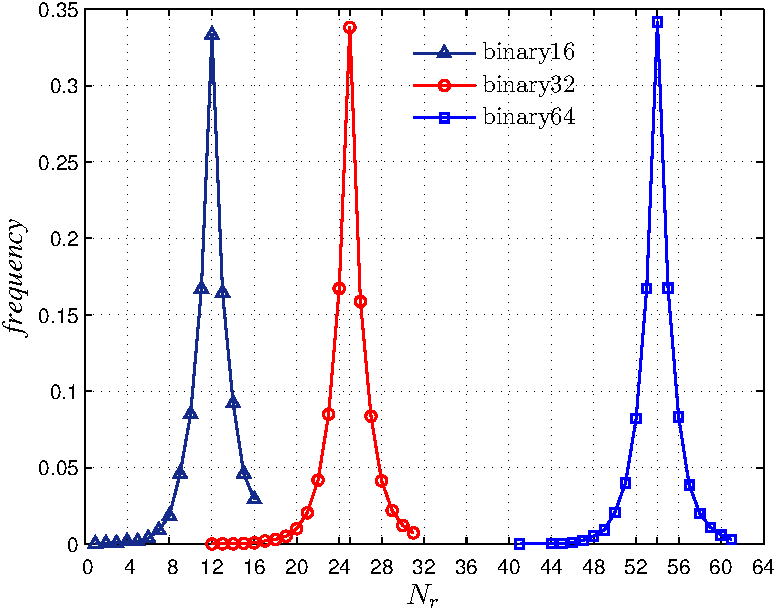
\includegraphics[width=1.25\BigOneImW]{DL_binary}
\end{minipage}
\caption{$N_r$的不同值的出现频率}
\label{fig:DistributionL_binary}
\end{figure}

因为$N_r=L+1$,所以$E(N_r)=E(L)+1$。在计算机上随机进行10000次实验,可以看到,$N_r$的分布由运算环境决定。
图~\ref{fig:DistributionL_binary}中三条曲线分别表示binary16,binary32,binary64环境下$N_r$的分布规律,
其均值分别为11.95,24.97,54.01,这与~(\ref{eq:EL})式计算产生的理论值一致。

\section{不同域上混沌映射状态网络之间的关系}

根据浮点数在计算机中的表示形式可知,数与数之间的最小间隔为$2^{( 1- (2^{l-1}-1) )} \cdot 2^{-m} = 2^{2-2^{l-1}-m}$。
在精度为$n$的定点运算域上,数与数之间的间隔为$2^{-n}$。如果$2^{2-2^{l-1}-m}=2^{-n}$, 即$n=m+2^{l-1}-2$,
那么基于不同运算环境实现的混沌映射,其对应的状态映射网络有强相关性。

\begin{figure}[!htb]
\centering
\begin{minipage}{1.15\BigOneImW}
\centering
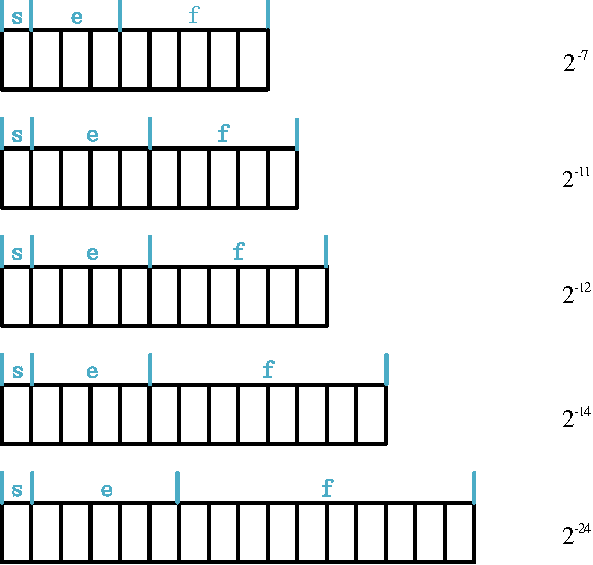
\includegraphics[width=1.15\BigOneImW]{float_point_format5}
\end{minipage}
\caption{浮点数在计算机中的表示形式及数与数之间的最小间隔}
\label{fig:float_point_format5}
\end{figure}

\begin{theorem}
给定二进制浮点格式参数$l$,$m$,则$F_{l,m}$中节点$i$和$F_{n}$中节点$i$满足关系
\begin{eqnarray}
F_{n}(i)- F_{l, m}(i)
\le
\begin{cases}
1               &  F_{n}(i)\in [0,2^{m});    \\
2^{n-m-1-j}     &  F_{n}(i)\in [2^{n-j-1},2^{n-j}),
\end{cases}
\end{eqnarray}
其中$j\in \{2^{l-1}-3, 2^{l-1}-4, \cdots, 1, 0\}$,且
\begin{equation}
\label{condition}
n = m+2^{l-1}-2.
\end{equation}
\label{theorem:fixedFloat}
\end{theorem}
\begin{proof}
因为$|x-\mathrm{R}(y)|= |\mathrm{R}(x-y)|,\ x\in \mathbb{Z}, y\in \mathbb{R}$,所以
\begin{eqnarray}
\left|F_{l,m}(i)-F_n(i)\right|
&=& \left|f_{l,m}(i) \cdot 2^{n}-\mathrm{R}\left(f_n(i) \cdot 2^{n}\right)\right|\nonumber\\
&=& \left| \mathrm{R}\left((f_{l,m}(i)-f_{n}(i))\cdot 2^{n}\right) \right|,
\label{eq:xRy}
\end{eqnarray}
其中$F_{l, m}(i)=f_{l,m}(i) \cdot 2^{n}$。

对SMN\ $F_{n}$中节点``$i$",其对应值$i/2^n$可在计算机内存中准确表示。不失一般性,假设在定点和浮点运算域上
$f(i/2^n)$的中间运算或处理过程相同,$f_{l, m}(i)$与$f_{n}(i)$的差值仅由最终量化误差引起。
当$F_{n}(i)\in [2^{n-1-j}, 2^{n-j})$时,有
\begin{align}
f_{l, m}(i)       =&  2^{-j-1}\cdot \left(1+\sum_{i=1}^m a_i \cdot 2^{-i} \right),\\
f_{n}(i)          =&  2^{-j-1}\cdot \left(1+\sum_{i=1}^n c_i \cdot 2^{-i} \right),
\end{align}
其中$j\in \{0, \cdots, 2^{l-1}-3\}$,对任意$i\in \{1,2,\cdots,m\}$,$a_i=c_i$。根据上述条件,进一步可推得
\begin{align}
f_{n}(i)-f_{l, m}(i) = 2^{-j-1}\cdot \left( \sum_{i=m+1}^n c_i \cdot 2^{-i} \right) < 2^{-m-j-1}.
\label{eq:nlmJ}
\end{align}
将~(\ref{eq:nlmJ})式代入~(\ref{eq:xRy})式,则有
\begin{eqnarray}
F_n(i)- F_{l,m}(i)
& =   & \mathrm{R}\left( ( f_{n}(i)-f_{l,m}(i) )\cdot 2^{m+1+j}
                \cdot 2^{n-m-1-j}\right)\nonumber\\
& \le & \mathrm{R}\left(2^{n-m-1-j}\right)
= 2^{n-m-1-j}.
\end{eqnarray}
当$F_{n}(i)\in [0, 2^{m})$时,$f_{l,m}(i)$为非规格化数,$f_{l,m}(i)$和$f_{n}(i)$可分别表示为
\begin{align}
f_{l, m}(i)       =&  2^{2-2^{l-1}}\cdot \left( \sum_{i=1}^m a_i \cdot 2^{-i} \right),\\
f_{n}(i)          =&  2^{2-2^{l-1}}\cdot \left( \sum_{i=1}^n c_i \cdot 2^{-i} \right).
\end{align}

\begin{figure}[!htb]
\centering
\begin{minipage}{0.98\BigTwoImW}
\centering
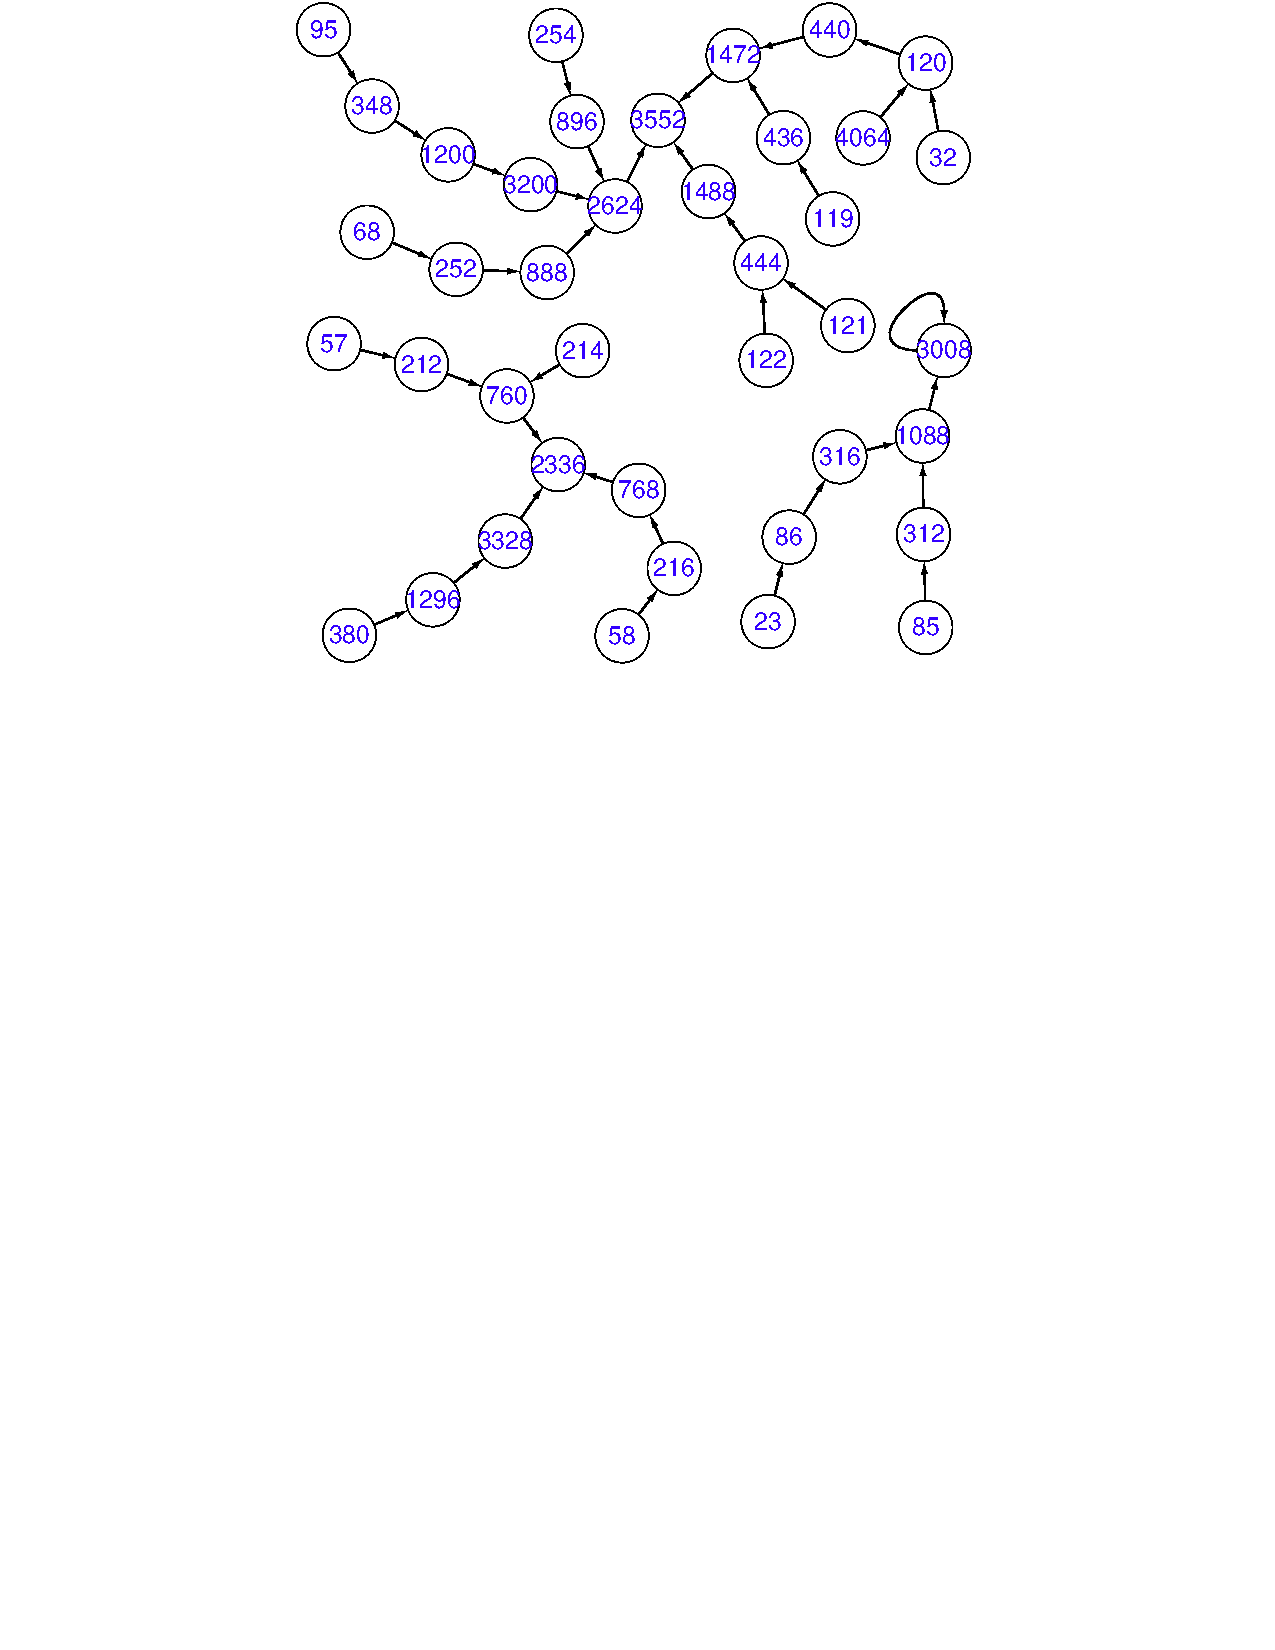
\includegraphics[width=0.98\BigTwoImW]{11bit_out_index_data_part}
a)
\end{minipage}\hspace{\figsep}
\hspace{1mm}
\begin{minipage}{\BigTwoImW}
\centering
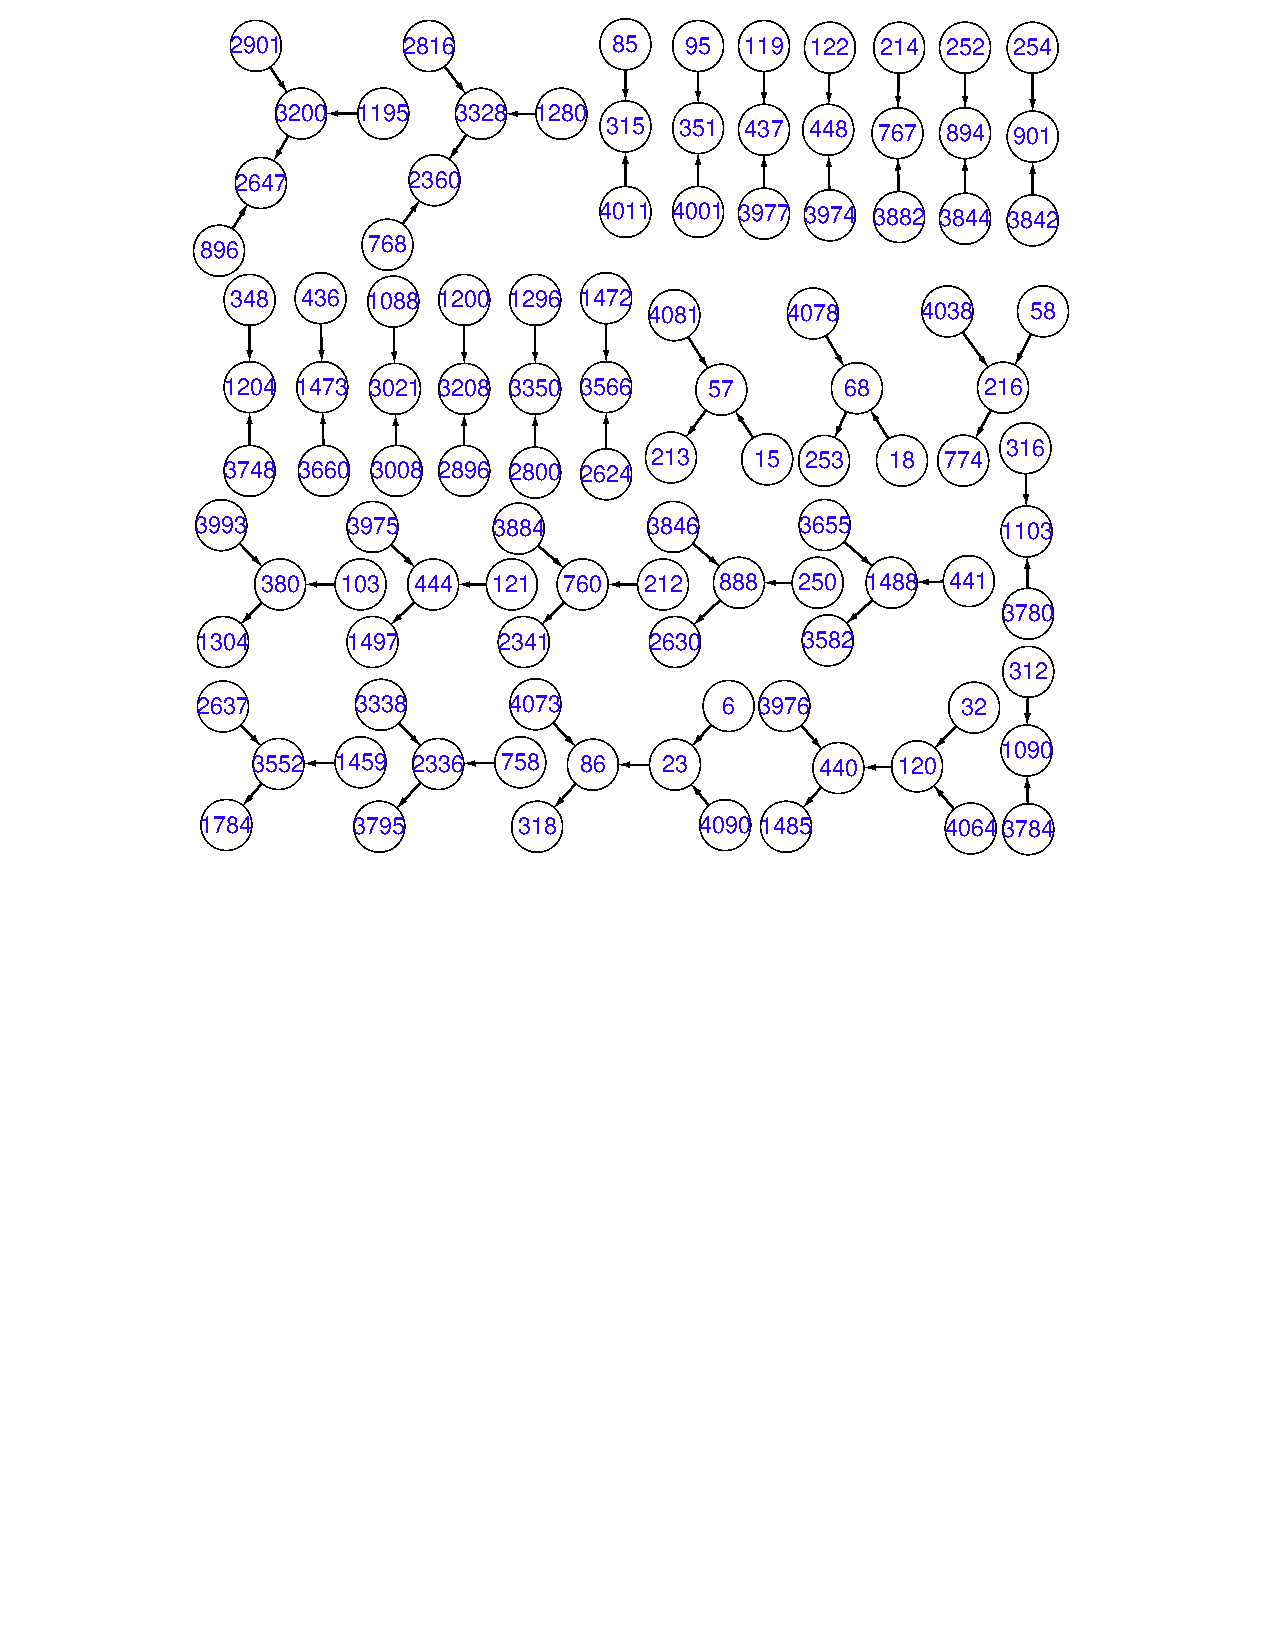
\includegraphics[width=\BigTwoImW]{12bit_precision_value_index_part}
b)
\end{minipage}
\caption{控制参数$\mu=121/2^5$时,浮点运算域上Logistic映射的状态映射网络的连通分量及对应定点运算域上其状态映射网络节点间的相对关系:
a) $(l,m)=(4,6)$; b) $n=12$}
\label{fig:networklogistic12and11bits}
\end{figure}

\begin{table}[!htb]
\centering
\caption{定点和浮点运算域上Logistic映射的状态映射网络部分对应节点的差值}
\resizebox{\textwidth}{26mm}{
\begin{tabular}{c *{9}{|c}}
\hline
$i$ & $F_{n}(i)$ & $F_{l,m}(i)$ & $\left|F_{n}(i)-F_{l,m}(i)\right|$ & $2^{n-m-1-j}$ &
$i$ & $F_{n}(i)$ & $F_{l,m}(i)$ & $\left|F_{n}(i)-F_{l,m}(i)\right|$ & $2^{n-m-1-j}$\\ \hline
6    & 23   & 22   & 1  & 1  & 156  & 567  & 560  & 7  & 8  \\ \hline
18   & 68   & 67   & 1  & 1  & 238  & 848  & 840  & 8  & 8  \\ \hline
33   & 124  & 123  & 1  & 1  & 284  & 999  & 992  & 7  & 8  \\ \hline
40   & 150  & 148  & 2  & 2  & 316  & 1103 & 1088 & 15 & 16 \\ \hline
53   & 198  & 196  & 2  & 2  & 576  & 1872 & 1856 & 16 & 16 \\ \hline
67   & 249  & 248  & 2  & 2  & 648  & 2063 & 2048 & 15 & 16 \\ \hline
82   & 304  & 300  & 4  & 4  & 768  & 2360 & 2336 & 24 & 32 \\ \hline
112  & 412  & 408  & 4  & 4  & 1280 & 3328 & 3296 & 32 & 32 \\ \hline
130  & 476  & 472  & 4  & 4  & 2080 & 3871 & 3840 & 31 & 32 \\ \hline
\end{tabular}}
\label{tab:difference}
\end{table}
类似地,可推得
\begin{align}
f_{n}(i)-f_{l, m}(i) =  2^{2-2^{l-1}}\cdot \left(\sum_{i=m+1}^n c_i \cdot 2^{-i}\right) < 2^{-m+2-2^{l-1}} = 2^{-n}.
\label{eq:nlmL}
\end{align}
根据~(\ref{eq:nlmL})式,进一步有
\begin{align}
\left|F_{l,m}(i)-F_n(i)\right| = \mathrm{R}\left(\left| (f_{l,m}(i)-f_{n}(i))\cdot 2^{n} \right|\right) \le \mathrm{R}\left(1\right)= 1.
\end{align}\qedsymbol
\end{proof}

\begin{table*}[!htb]
\centering
\caption{定点和浮点运算域上Tent映射的状态映射网络部分对应节点的差值}
\resizebox{\textwidth}{28mm}{
\begin{tabular}{c *{7}{|c}}
\hline
$i$ & $F_{n}(i)$ & $f_{n}(i)-f_{l,m}(i)$  & $2^{-(m+1+j)}$ & $i$ & $F_{n}(i)$ & $f_{n}(i)-f_{l,m}(i)$  & $2^{-(m+1+j)}$\\ \hline
17 & 32 & 0.013671875  & 0.03125  & 34 & 56 & 0.00390625   & 0.03125  \\ \hline
19 & 36 & 0.025390625  & 0.03125  & 38 & 49 & 0.01171875   & 0.03125  \\ \hline
21 & 39 & 0.021484375  & 0.03125  & 42 & 41 & 0.01953125   & 0.03125  \\ \hline
23 & 43 & 0.017578125  & 0.03125  & 46 & 34 & 0.02734375   & 0.03125  \\ \hline
25 & 47 & 0.013671875  & 0.03125  & 50 & 26 & 0.00390625   & 0.015625 \\ \hline
27 & 51 & 0.009765625  & 0.03125  & 54 & 19 & 0.01171875   & 0.015625 \\ \hline
29 & 54 & 0.005859375  & 0.03125  & 58 & 11 & 0.00390625   & 0.015625 \\ \hline
31 & 58 & 0.001953125  & 0.03125  & 62 & 4  & 0.01171875   & 0.015625 \\ \hline
\end{tabular}}
\label{tab:realdifftent}
\end{table*}

图~\ref{fig:networklogistic12and11bits} a)为定点运算域上Logistic映射的状态映射网络$F_{12}$的其中三个连通分量,
图~\ref{fig:networklogistic12and11bits} b)为浮点运算域上Logistic映射的状态映射网络$F_{4, 6}$节点间的相对关系,
图~\ref{fig:networklogistic12and11bits} b)为图~\ref{fig:networklogistic12and11bits} a)中对应节点及其邻接点。
表~\ref{tab:difference}给出Logistic映射SMN\ $F_{12}$与SMN\ $F_{4, 6}$部分对应节点的差值及其理论值,Logistic映射
的控制参数$\mu=121/2^5$,浮点运算模式下浮点数格式参数$(l,m)=(4,6)$,定点运算精度$n=12$。
表~\ref{tab:realdifftent}列出Tent映射SMN\ $F_{6}$与SMN\ $F_{3, 4}$部分对应节点的差值及其理论值,Tent映射的控制
参数$\mu=15/2^4$,浮点运算模式下浮点数格式参数$(l,m)=(3,4)$,定点运算精度$n=6$。
\iffalse Tent映射的SMN\ $F_{3, 4}$和SMN\ $F_{6}$如图~\ref{fig:networkTent8and6bits}所示。\fi
这里$f_{l,m}(i)$由低精度浮点运算模拟器计算得到,其中$i\in \{0, \cdots, 2^n\}$。
从这些仿真数据又可以进一步检验定理~\ref{theorem:fixedFloat}的正确性。

根据定理~\ref{theorem:fixedFloat}可知,浮点运算域上混沌映射的状态映射网络可以看作定点运算域上其对应状态映射网络的子网络重构。
更准确地说,SMN\ $F_{l,m}$可由SMN\ $F_{n}$生成,当$2^{n-j}-(k+1)\cdot 2^{n-m-1-j} < F_{n}(i) < 2^{n-j}-k\cdot 2^{n-m-1-j}$时,
指向$F_{n}(i)$的所有节点重新指向节点$2^{n-j}-(k+1)\cdot 2^{n-m-1-j}$;当$F_{n}(i)= 2^{n-j}-k\cdot 2^{n-m-1-j}$时,
除节点$``2^{n}"$,指向$F_{n}(i)$的其余节点重新指向节点$2^{n-j}-k\cdot 2^{n-m-1-j}$和$2^{n-j}-(k+1)\cdot 2^{n-m-1-j}$,
$j\in \{2^{l-1}-4, \cdots, 1, 0\}$,$k=0\sim 2^{m}-1$;当$0 < F_{n}(i) < 2^{m+1}$时,指向$F_{n}(i)$的所有节点
重新指向节点$F_{n}(i)$和$F_{n}(i)-1$。
SMN\ $F_{l,m}$生成过程可以通过分析图~\ref{fig:networkLogistic8and6bits}和图~\ref{fig:networkTent8and6bits}进一步验证。

\begin{figure}[!htb]
\centering
\begin{minipage}{\TwoImW}
\centering
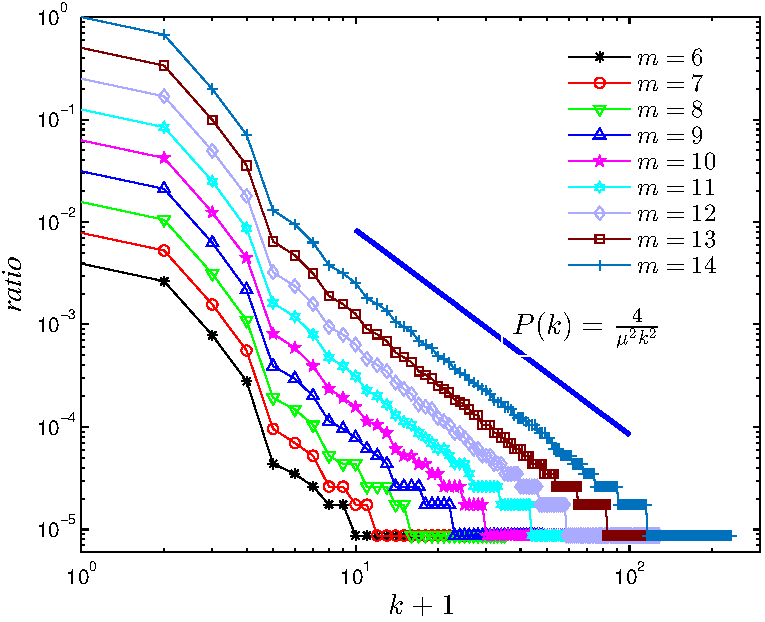
\includegraphics[width=\TwoImW]{CumulativeInDegreeDistribution_FloatingPointExponent4}
a)
\end{minipage}
\begin{minipage}{\TwoImW}
\centering
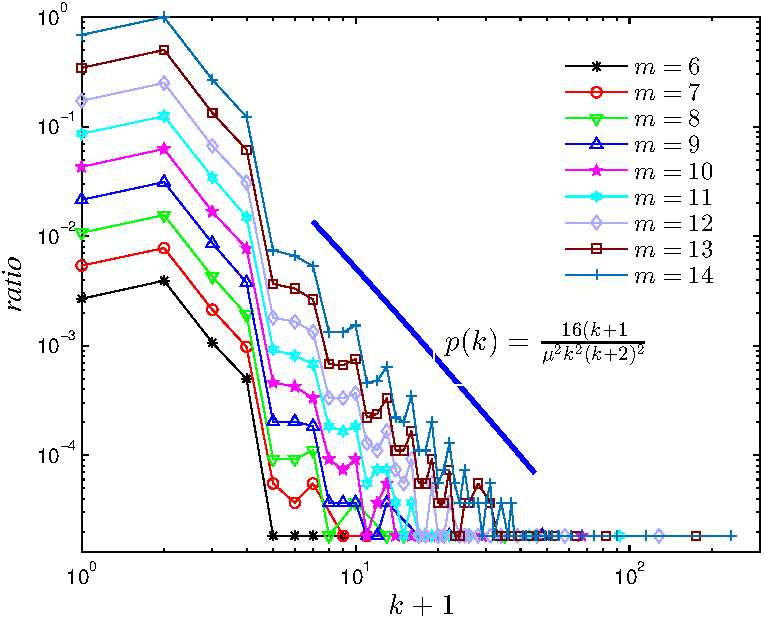
\includegraphics[width=\TwoImW]{InDegreeDistribution_FloatingPointExponent4}
b)
\end{minipage}
\caption{浮点运算域上Logistic映射的状态映射网络的节点累积入度分布和入度分布}
\label{fig:CumulativeInDegreeDistribution4}
\end{figure}

\begin{figure}[!htb]
\centering
\begin{minipage}{\BigTwoImW}
\centering
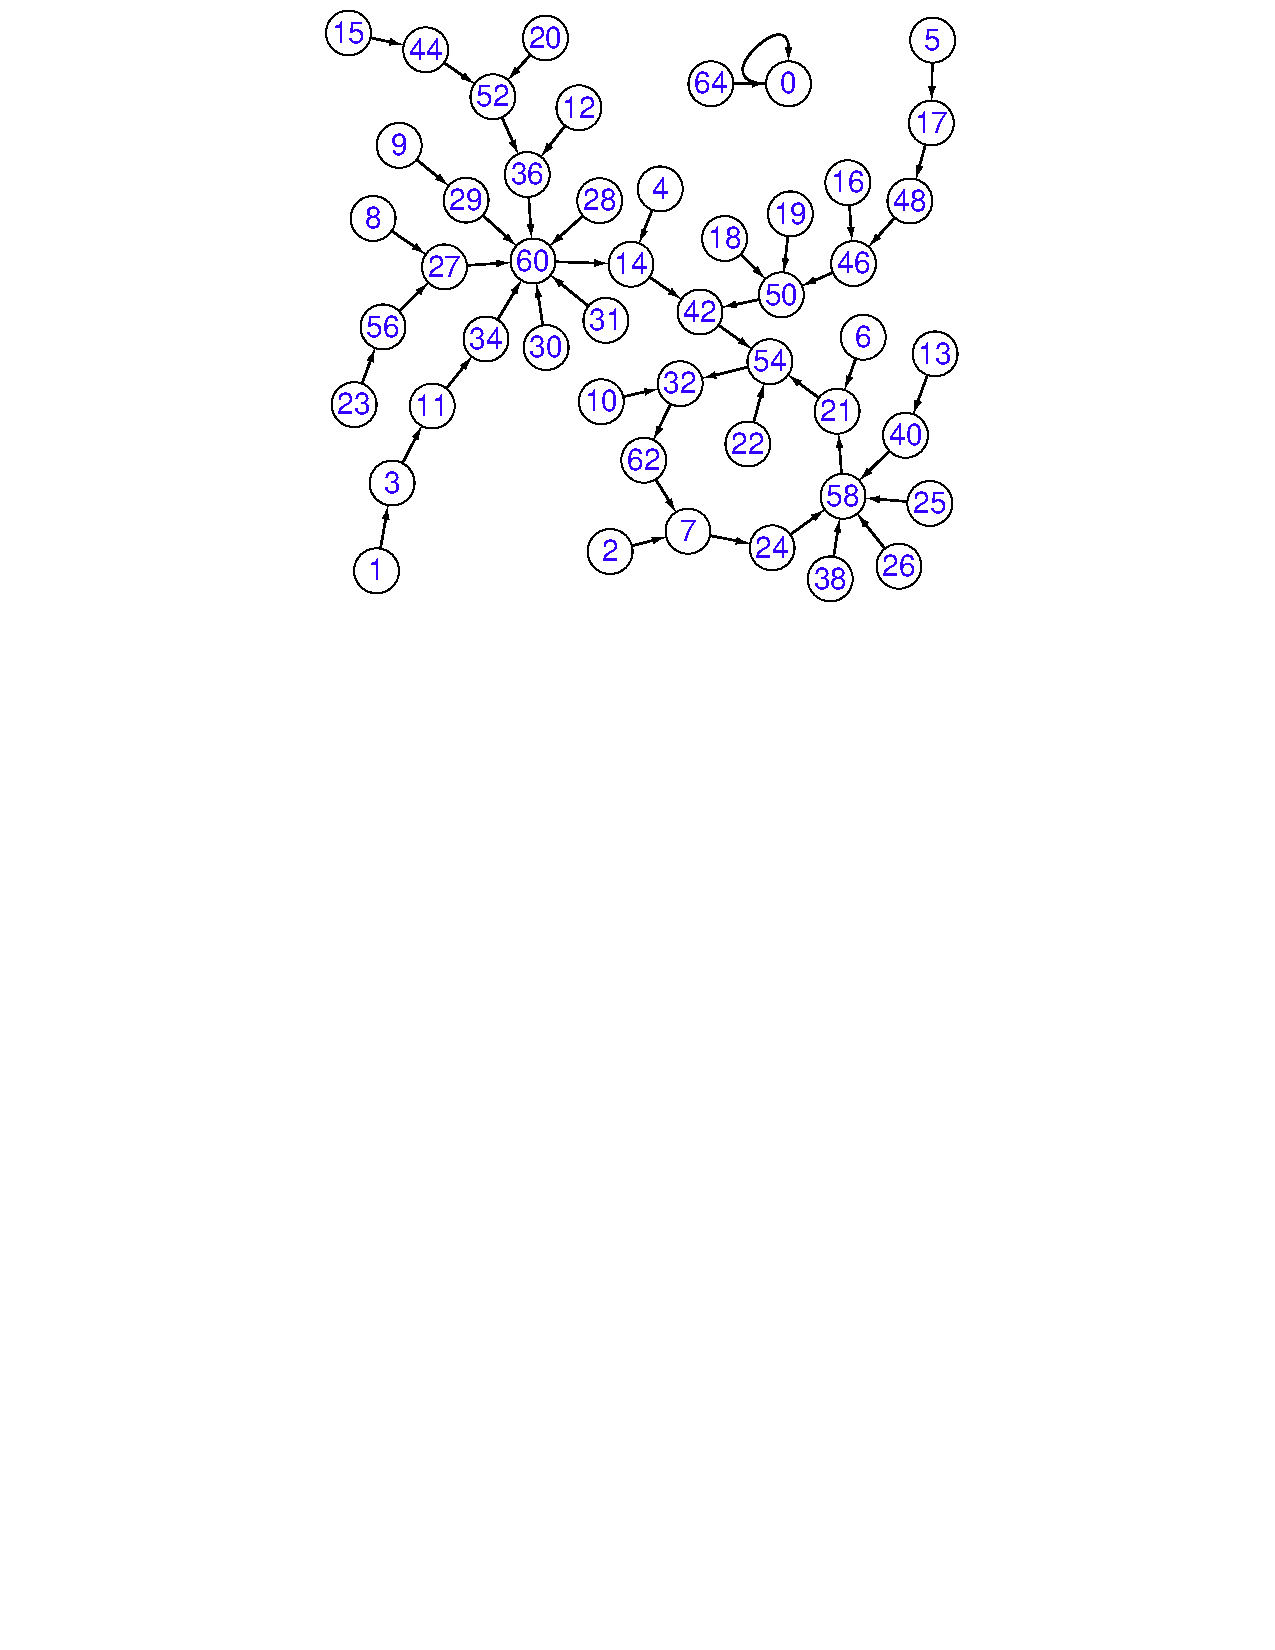
\includegraphics[width=\BigTwoImW]{8bit_out_index_data_u3875}
a)
\end{minipage}  \hspace{\figsep}
\begin{minipage}{0.98\BigTwoImW}
\centering
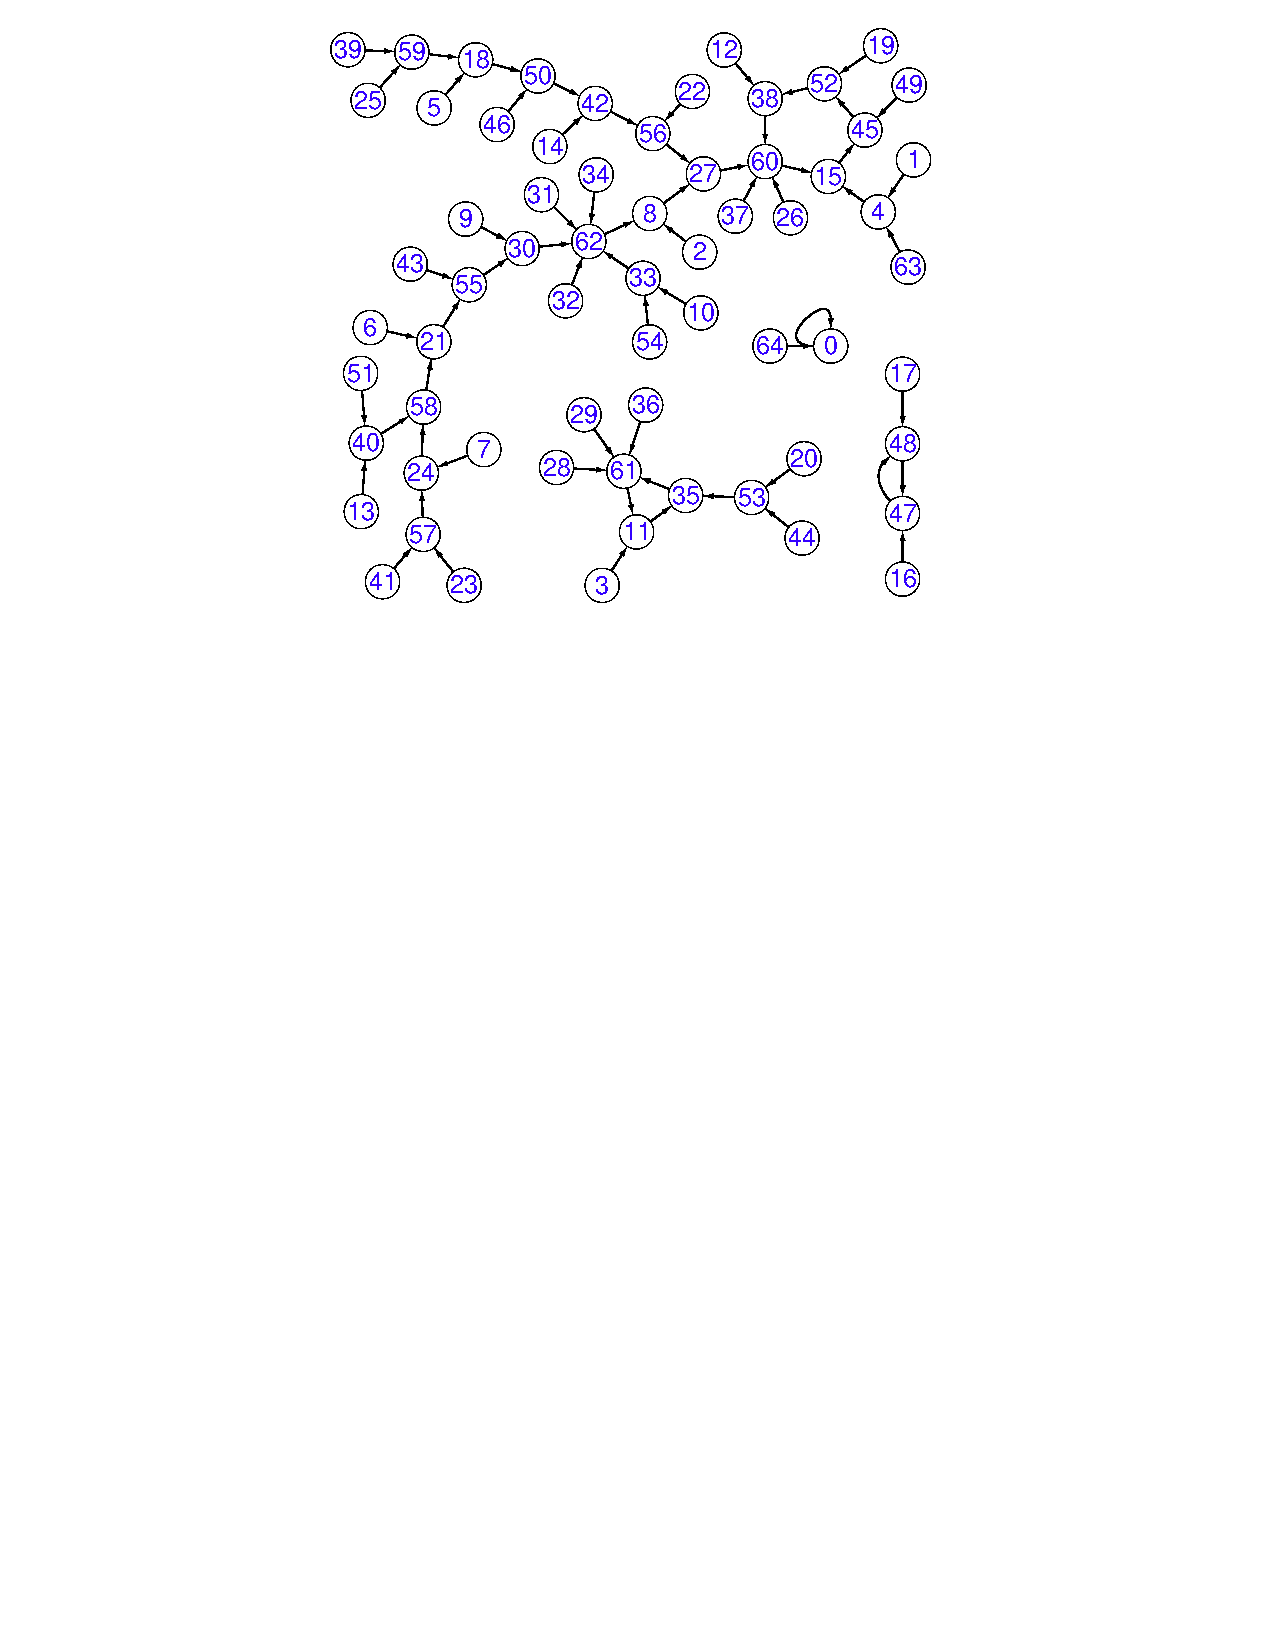
\includegraphics[width=0.98\BigTwoImW]{6bit_precision_value_index_u3875}
b)
\end{minipage}
\caption{控制参数$\mu=62/2^4$时,Logistic映射的状态映射网络:
a) $(l,m)=(3,4)$; b) $n=6$}
\label{fig:networkLogistic8and6bits}
\end{figure}

\begin{figure}[!htb]
\centering
\begin{minipage}{0.97\BigTwoImW}
\centering
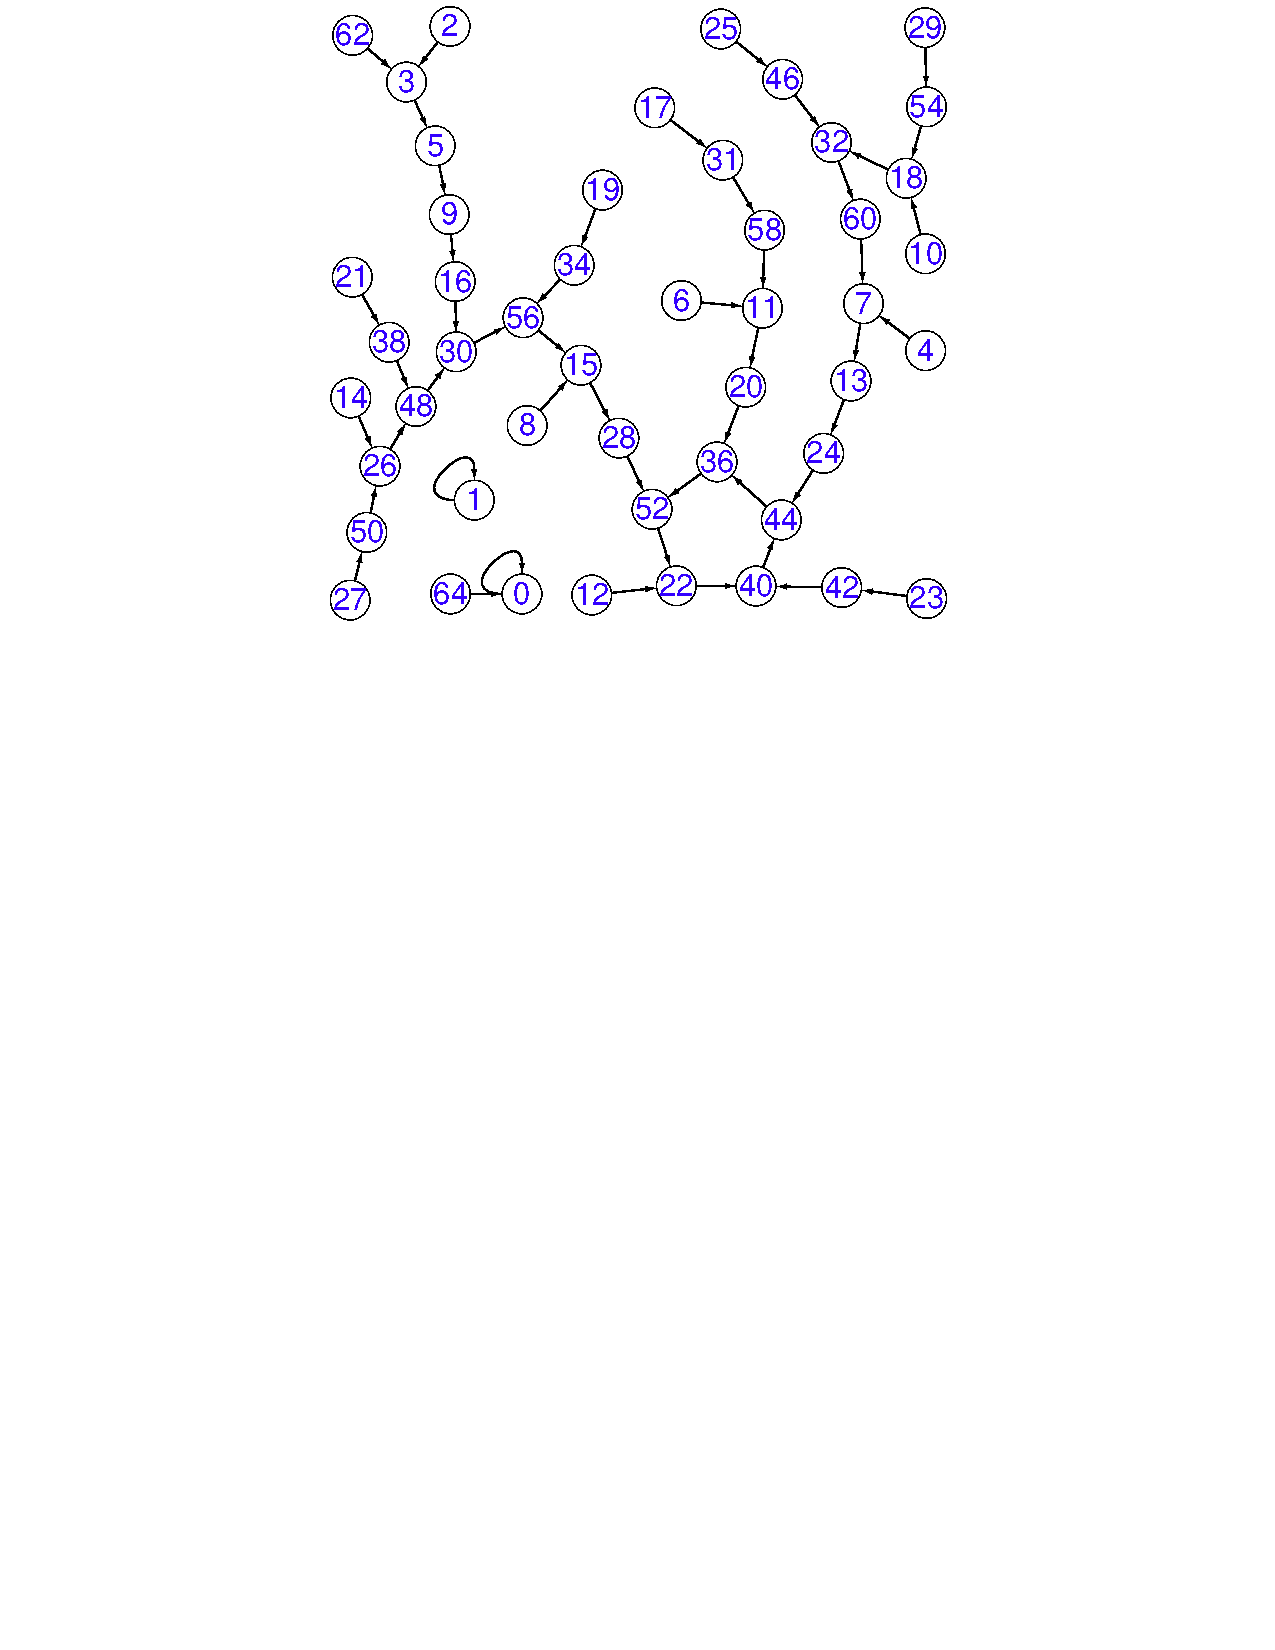
\includegraphics[width=0.97\BigTwoImW]{8bit_out_index_data_tent_u09375}
a)
\end{minipage}\hspace{\figsep}
\begin{minipage}{\BigTwoImW}
\centering
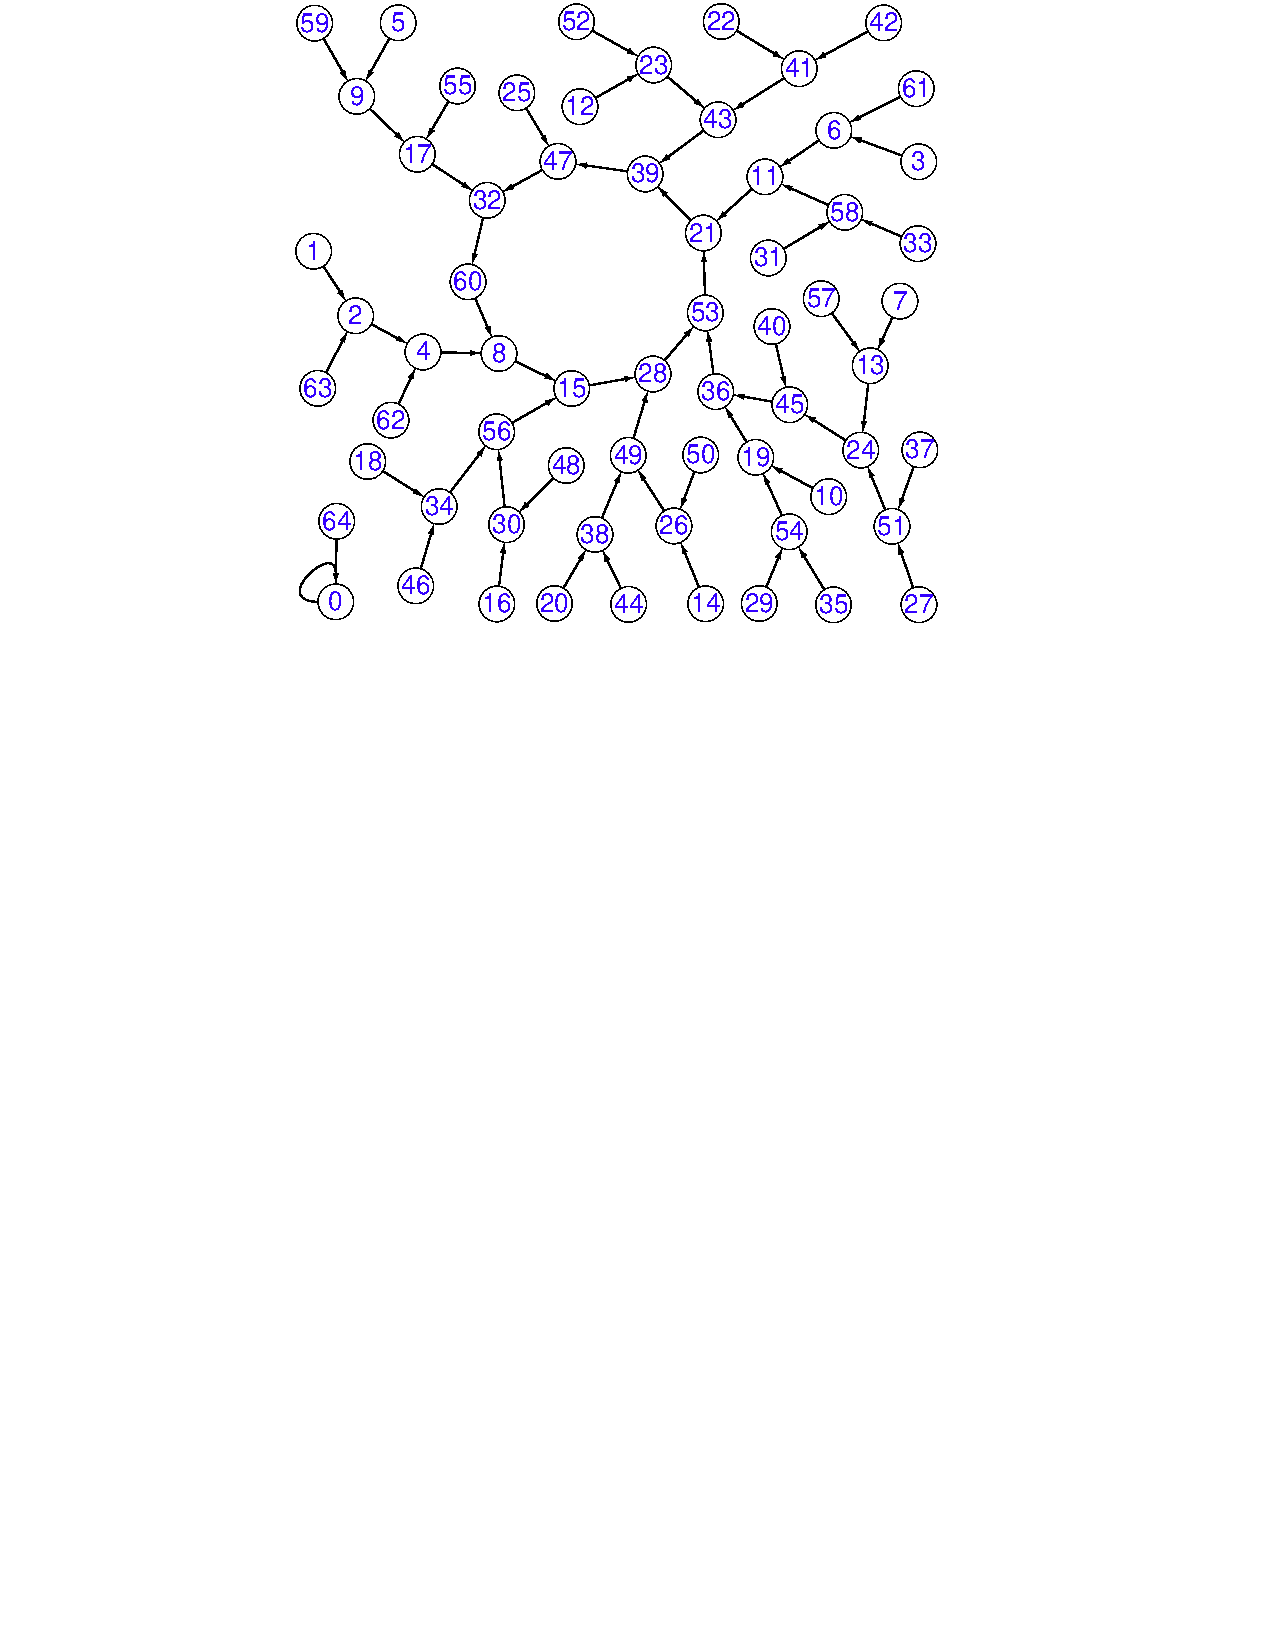
\includegraphics[width=\BigTwoImW]{6bit_precision_value_index_tent_u09375}
b)
\end{minipage}
\caption{控制参数$\mu=15/2^4$时,Tent映射的状态映射网络:
a) $(l,m)=(3,4)$; b) $n=6$}
\label{fig:networkTent8and6bits}
\end{figure}

图~\ref{fig:CumulativeInDegreeDistribution4} a)为浮点运算域上Logistic映射的状态映射网络的节点累积入度分布,
图~\ref{fig:CumulativeInDegreeDistribution4} b)为其入度分布。
根据定理~\ref{theorem:logisticMap}和定理~\ref{theorem:fixedFloat}可知,
浮点运算域上Logistic映射的状态映射网络的节点累积入度分布和入度分布逼近对应定点运算域上其幂律分布。
上述讨论可以通过图~\ref{fig:CumulativeInDegreeDistribution_u121_n_5_20}、图~\ref{fig:InDegreeDistribution_u121_n_5_20}和图~\ref{fig:CumulativeInDegreeDistribution4}之间的对比分析进一步得到验证,这里$l=4$。


\section{本章小结}

本章讨论了数字计算机上分段线性混沌映射Tent映射的相关动力学性质,首先利用整数量化函数准确推导出了Tent映射的状态映射网络$F^*_{n}$与实现精度$n$之间的关系,
理论上证明了Tent映射的状态映射网络的节点入度取值范围;其次,严格证明了Tent映射的混沌轨道将在有限次迭代中收敛于零,其收敛于零的平均迭代次数和最大迭代次数由有关
数字运算的细节唯一决定,当初始条件$x(0)$在浮点域上均匀分布时,平均迭代次数通常比最大迭代次数要小得多。该结论可以直接推广到其他类似混沌映射,如
Bernoulli移位映射、V-映射、Baker映射;最后,初步揭示了定点和浮点运算域上混沌映射的状态映射网络$f_{n}$与$f_{l, m}$之间的关系,根据它们之间的
关系,对混沌系统的分析可能会变得容易一些。